\chapter{Travaux réalisés}

\section{Démarche et organisation du travail}

Le travail a suivi une démarche en trois temps : (1) documenter le besoin avant d'écrire du code, (2) concevoir l'architecture et le modèle de données, (3) développer fonctionnalité par fonctionnalité, en testant chaque règle métier.

\begin{itemize}
  \item \textbf{Documentation préalable} : vision, cahier des charges, objectifs, workflow, cas d'utilisation, architecture et base de données (documents Markdown versionnés dans le dépôt).
  \item \textbf{Gestion de version Git} : branche \texttt{main} stable, branche \texttt{develop} d'intégration, branches de fonctionnalité et messages de commit normalisés (Conventional Commits). Le dépôt compte 31 commits.
  \item \textbf{Développement piloté par les règles métier} : chaque règle (transition, unicité, permission) est couverte par un test automatisé.
\end{itemize}

Le déroulement du projet est reconstitué à partir des observations du stage et de l'historique du dépôt Git.

\Needspace{7\baselineskip}

{\small\setstretch{1.05}\renewcommand{\arraystretch}{1.3}\arrayrulecolor{ALtexte}
\begin{longtable}{|>{\raggedright\arraybackslash}p{4.11cm}|>{\raggedright\arraybackslash}p{10.50cm}|}
\caption{Déroulement du projet}\\
\hline
\rowcolor{ALbleu} \sffamily\bfseries\color{white} Période & \sffamily\bfseries\color{white} Activité \\ \hline
\endfirsthead
\caption[]{Déroulement du projet (suite)}\\
\hline
\rowcolor{ALbleu} \sffamily\bfseries\color{white} Période & \sffamily\bfseries\color{white} Activité \\ \hline
\endhead
1\textsuperscript{er} juillet – 1\textsuperscript{er} août 2026 (stage) & Immersion au service Maintenance : observation du circuit retour, désinfection, atelier et stockage ; échanges avec le responsable et les techniciens ; recueil du besoin à partir du journal papier (entrée du 14 juillet 2026), du classeur Google Sheets et du questionnaire de retour \\ \hline
\rowcolor{ALgris} 15 et 16 juillet 2026 & Rédaction de la documentation de conception (vision, cahier des charges, workflow, cas d'utilisation, architecture, base de données), structure du dépôt, projet Django \\ \hline
Octobre 2026 (14, 27 et 28) & Réalisation et consolidation de l'application : authentification, workflow complet, questionnaire de retour, journal, interface, tests et documentation \\ \hline
\end{longtable}
}

\subsection{Outils d'assistance utilisés}

Conformément à une démarche transparente, il est précisé que des assistants d'intelligence artificielle ont été utilisés comme outils de travail : un assistant conversationnel pour structurer la conception initiale (architecture, base de données, workflow), puis un assistant de programmation pour accélérer le développement et la rédaction des tests. L'étudiant a défini le besoin, pris les décisions de conception, relu, exécuté et validé le résultat.

\section{Analyse des besoins}

\Needspace{10\baselineskip}
\subsection{Acteurs}

{\small\setstretch{1.05}\renewcommand{\arraystretch}{1.3}\arrayrulecolor{ALtexte}
\begin{longtable}{|>{\raggedright\arraybackslash}p{3.56cm}|>{\raggedright\arraybackslash}p{4.00cm}|>{\raggedright\arraybackslash}p{6.67cm}|}
\caption{Acteurs et droits}\\
\hline
\rowcolor{ALbleu} \sffamily\bfseries\color{white} Acteur & \sffamily\bfseries\color{white} Rôle dans l'application & \sffamily\bfseries\color{white} Droits principaux \\ \hline
\endfirsthead
\caption[]{Acteurs et droits (suite)}\\
\hline
\rowcolor{ALbleu} \sffamily\bfseries\color{white} Acteur & \sffamily\bfseries\color{white} Rôle dans l'application & \sffamily\bfseries\color{white} Droits principaux \\ \hline
\endhead
Technicien de maintenance & Utilisateur principal de l'atelier & Enregistrer les retours, réaliser et valider chaque étape, consulter les fiches de vie et le journal \\ \hline
\rowcolor{ALgris} Responsable SAV & Supervision et administration & Tous les droits du technicien, plus : gestion des utilisateurs et des catalogues, rapports et exports, retour arrière d'un statut avec justification \\ \hline
\end{longtable}
}

\begin{figure}[p]
\centering
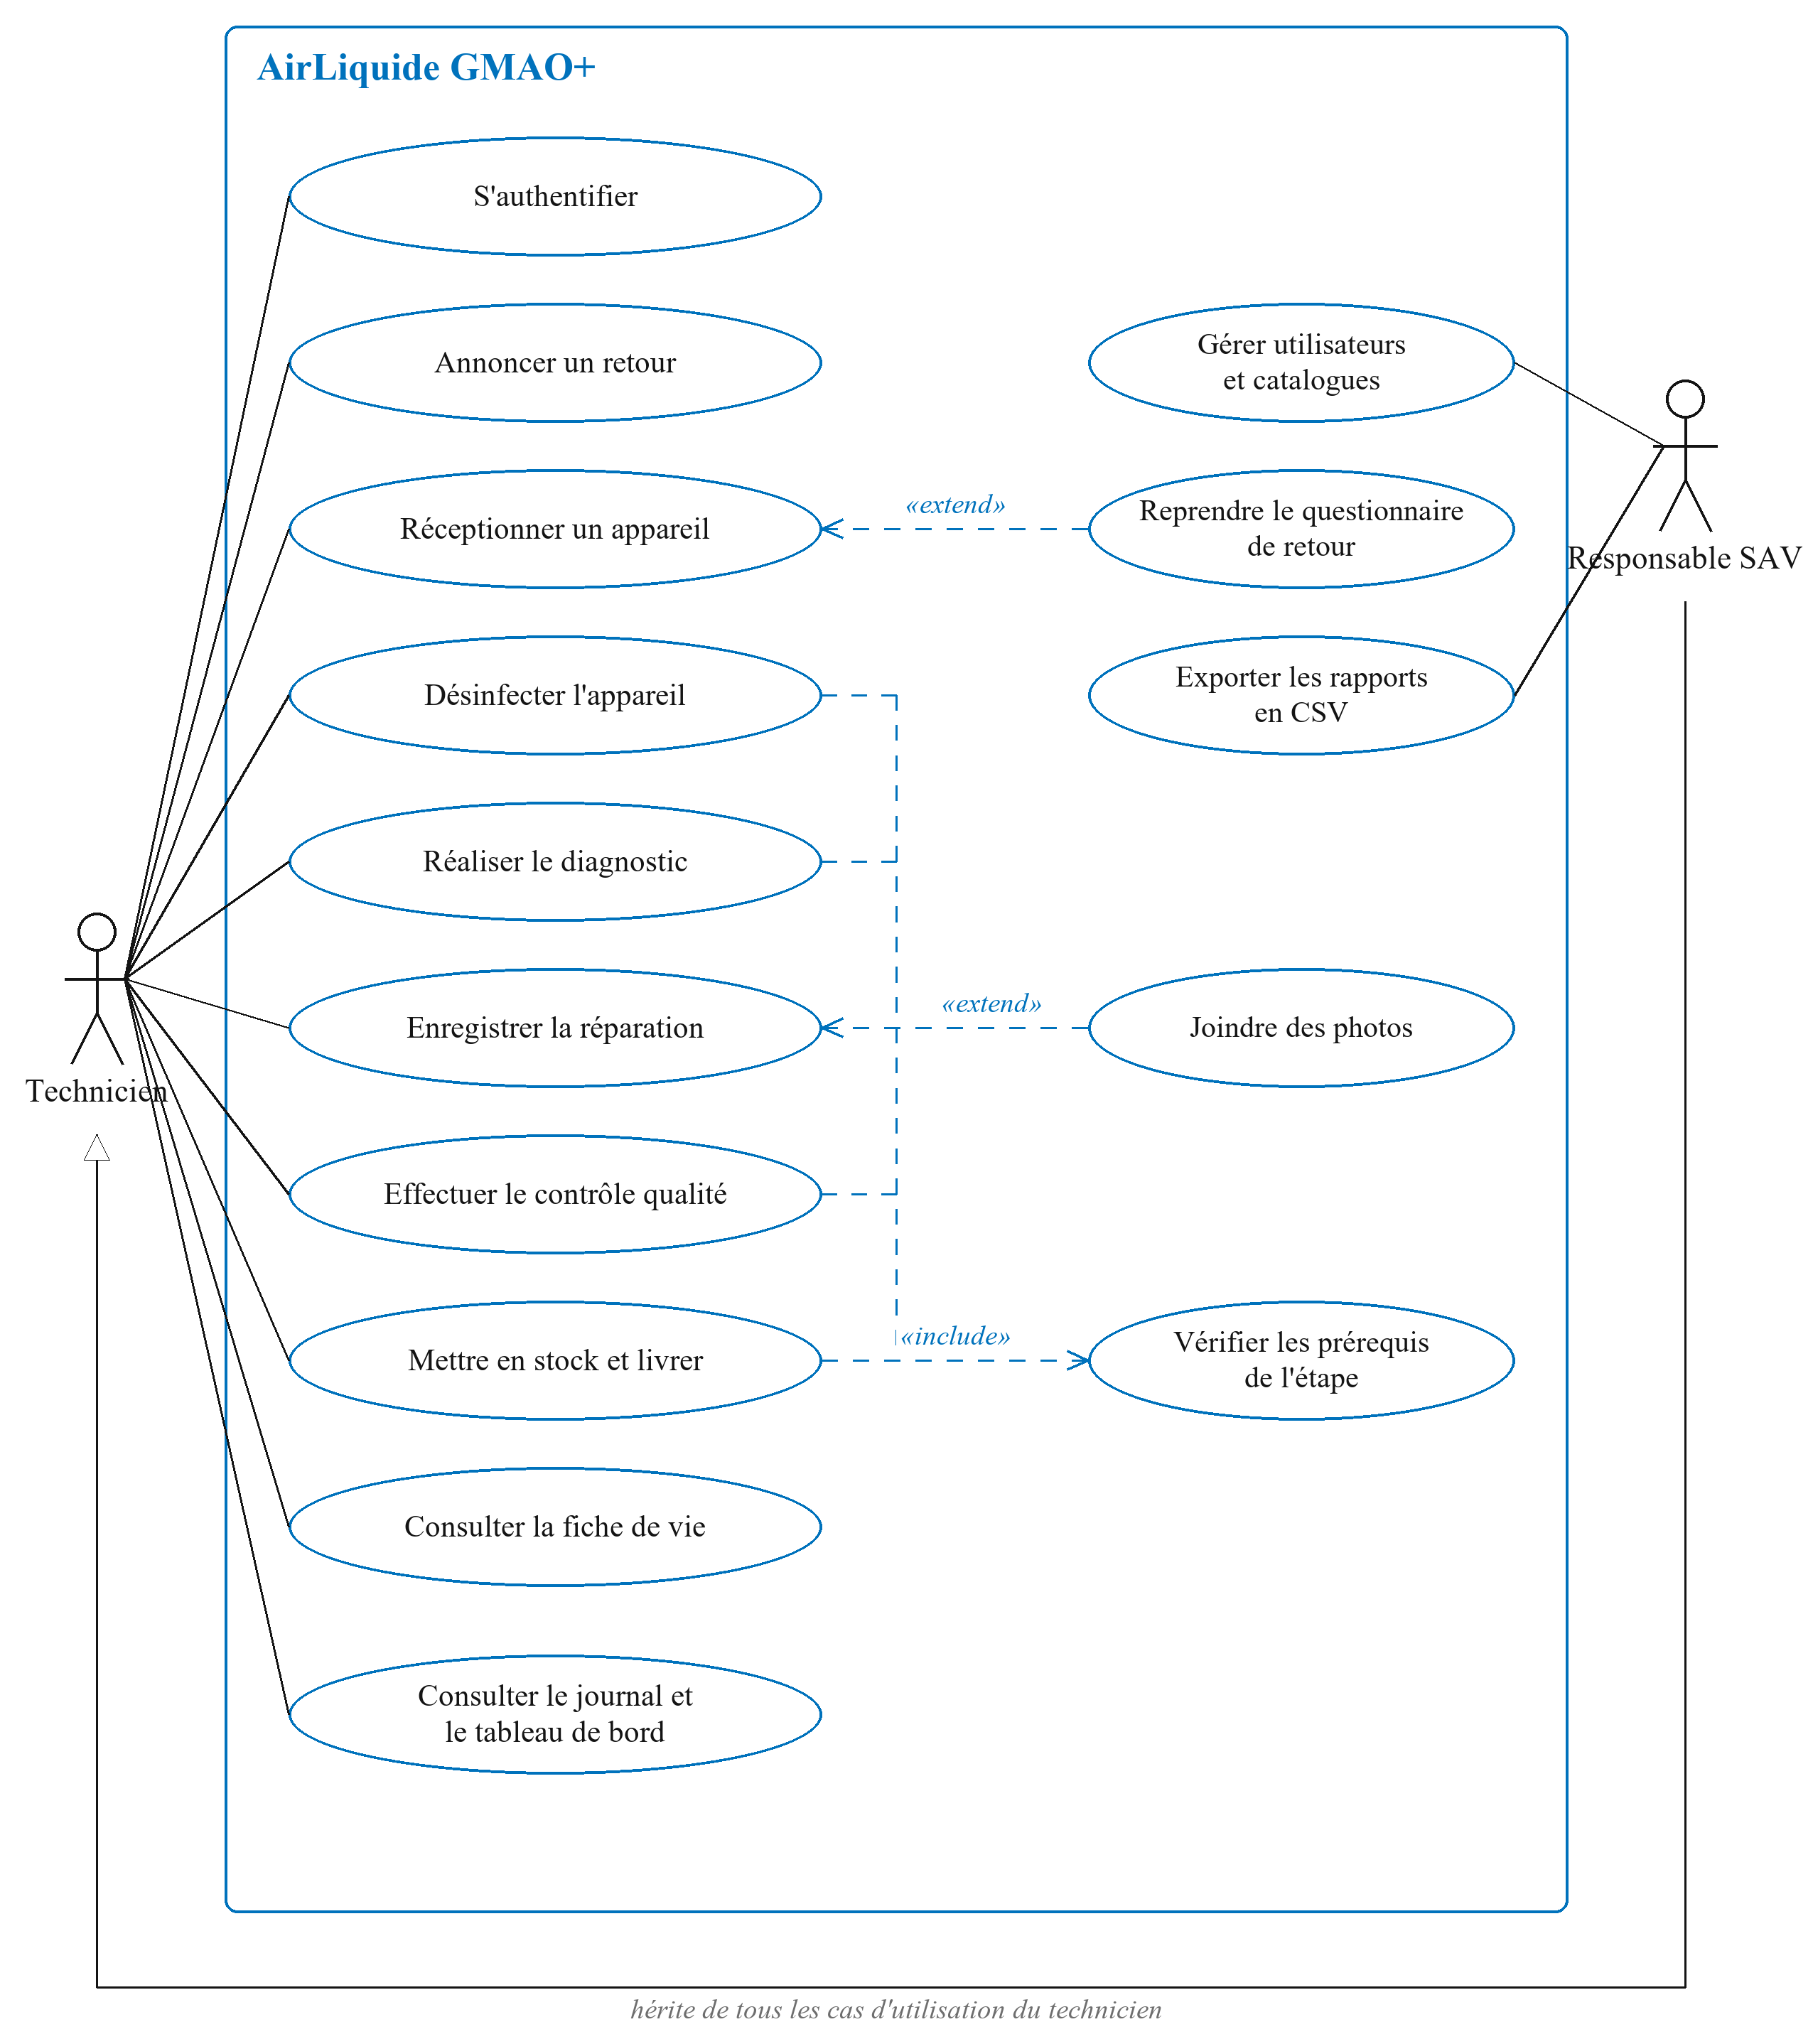
\includegraphics[width=15.5cm,height=18.5cm,keepaspectratio]{uml_cas_utilisation.png}
\caption{Diagramme de cas d'utilisation}
\end{figure}

Le Responsable SAV hérite de tous les cas d'utilisation du technicien et dispose en plus de la gestion des utilisateurs et des catalogues et de l'export des rapports. Chaque étape du workflow inclut la vérification de ses prérequis.

\subsection{Besoins fonctionnels}

\begin{itemize}
  \item annoncer un retour avant l'arrivée de l'appareil, puis le réceptionner ;
  \item retrouver un appareil par son numéro de série et consulter sa fiche de vie ;
  \item enregistrer la désinfection, le diagnostic (pannes d'un catalogue), la réparation (pièces, durée), le contrôle qualité (checklist et mesures), l'entrée en stock et la livraison ;
  \item joindre des photos aux dossiers ;
  \item consulter un tableau de bord et un journal de maintenance équivalent au registre papier ;
  \item exporter les données (CSV).
\end{itemize}

\subsection{Besoins non fonctionnels}

\begin{itemize}
  \item \textbf{Traçabilité} : chaque changement de statut conserve la date, l'heure et l'utilisateur ; l'historique ne peut être ni modifié ni supprimé ;
  \item \textbf{Sécurité} : authentification, permissions par rôle, validation des entrées côté serveur, protection des fichiers téléversés ;
  \item \textbf{Ergonomie} : interface en français, utilisable sur ordinateur et tablette, parcours courts pour les techniciens ;
  \item \textbf{Maintenabilité} : code modulaire, logique métier séparée des vues, tests automatisés.
\end{itemize}

\section{Conception}

Les diagrammes de cette section suivent la notation UML. Ils ont été dessinés pour ce rapport ; leurs sources textuelles équivalentes (PlantUML et Mermaid), versionnées avec le projet, se trouvent dans le dossier \texttt{docs/\allowbreak{}diagrams/\allowbreak{}}.

\subsection{Le workflow d'un appareil}

Le cycle de vie d'un appareil est modélisé par sept statuts successifs. Un dossier ne peut avancer que d'une étape à la fois, et seulement si l'étape correspondante a été enregistrée.

\begin{figure}[p]
\centering
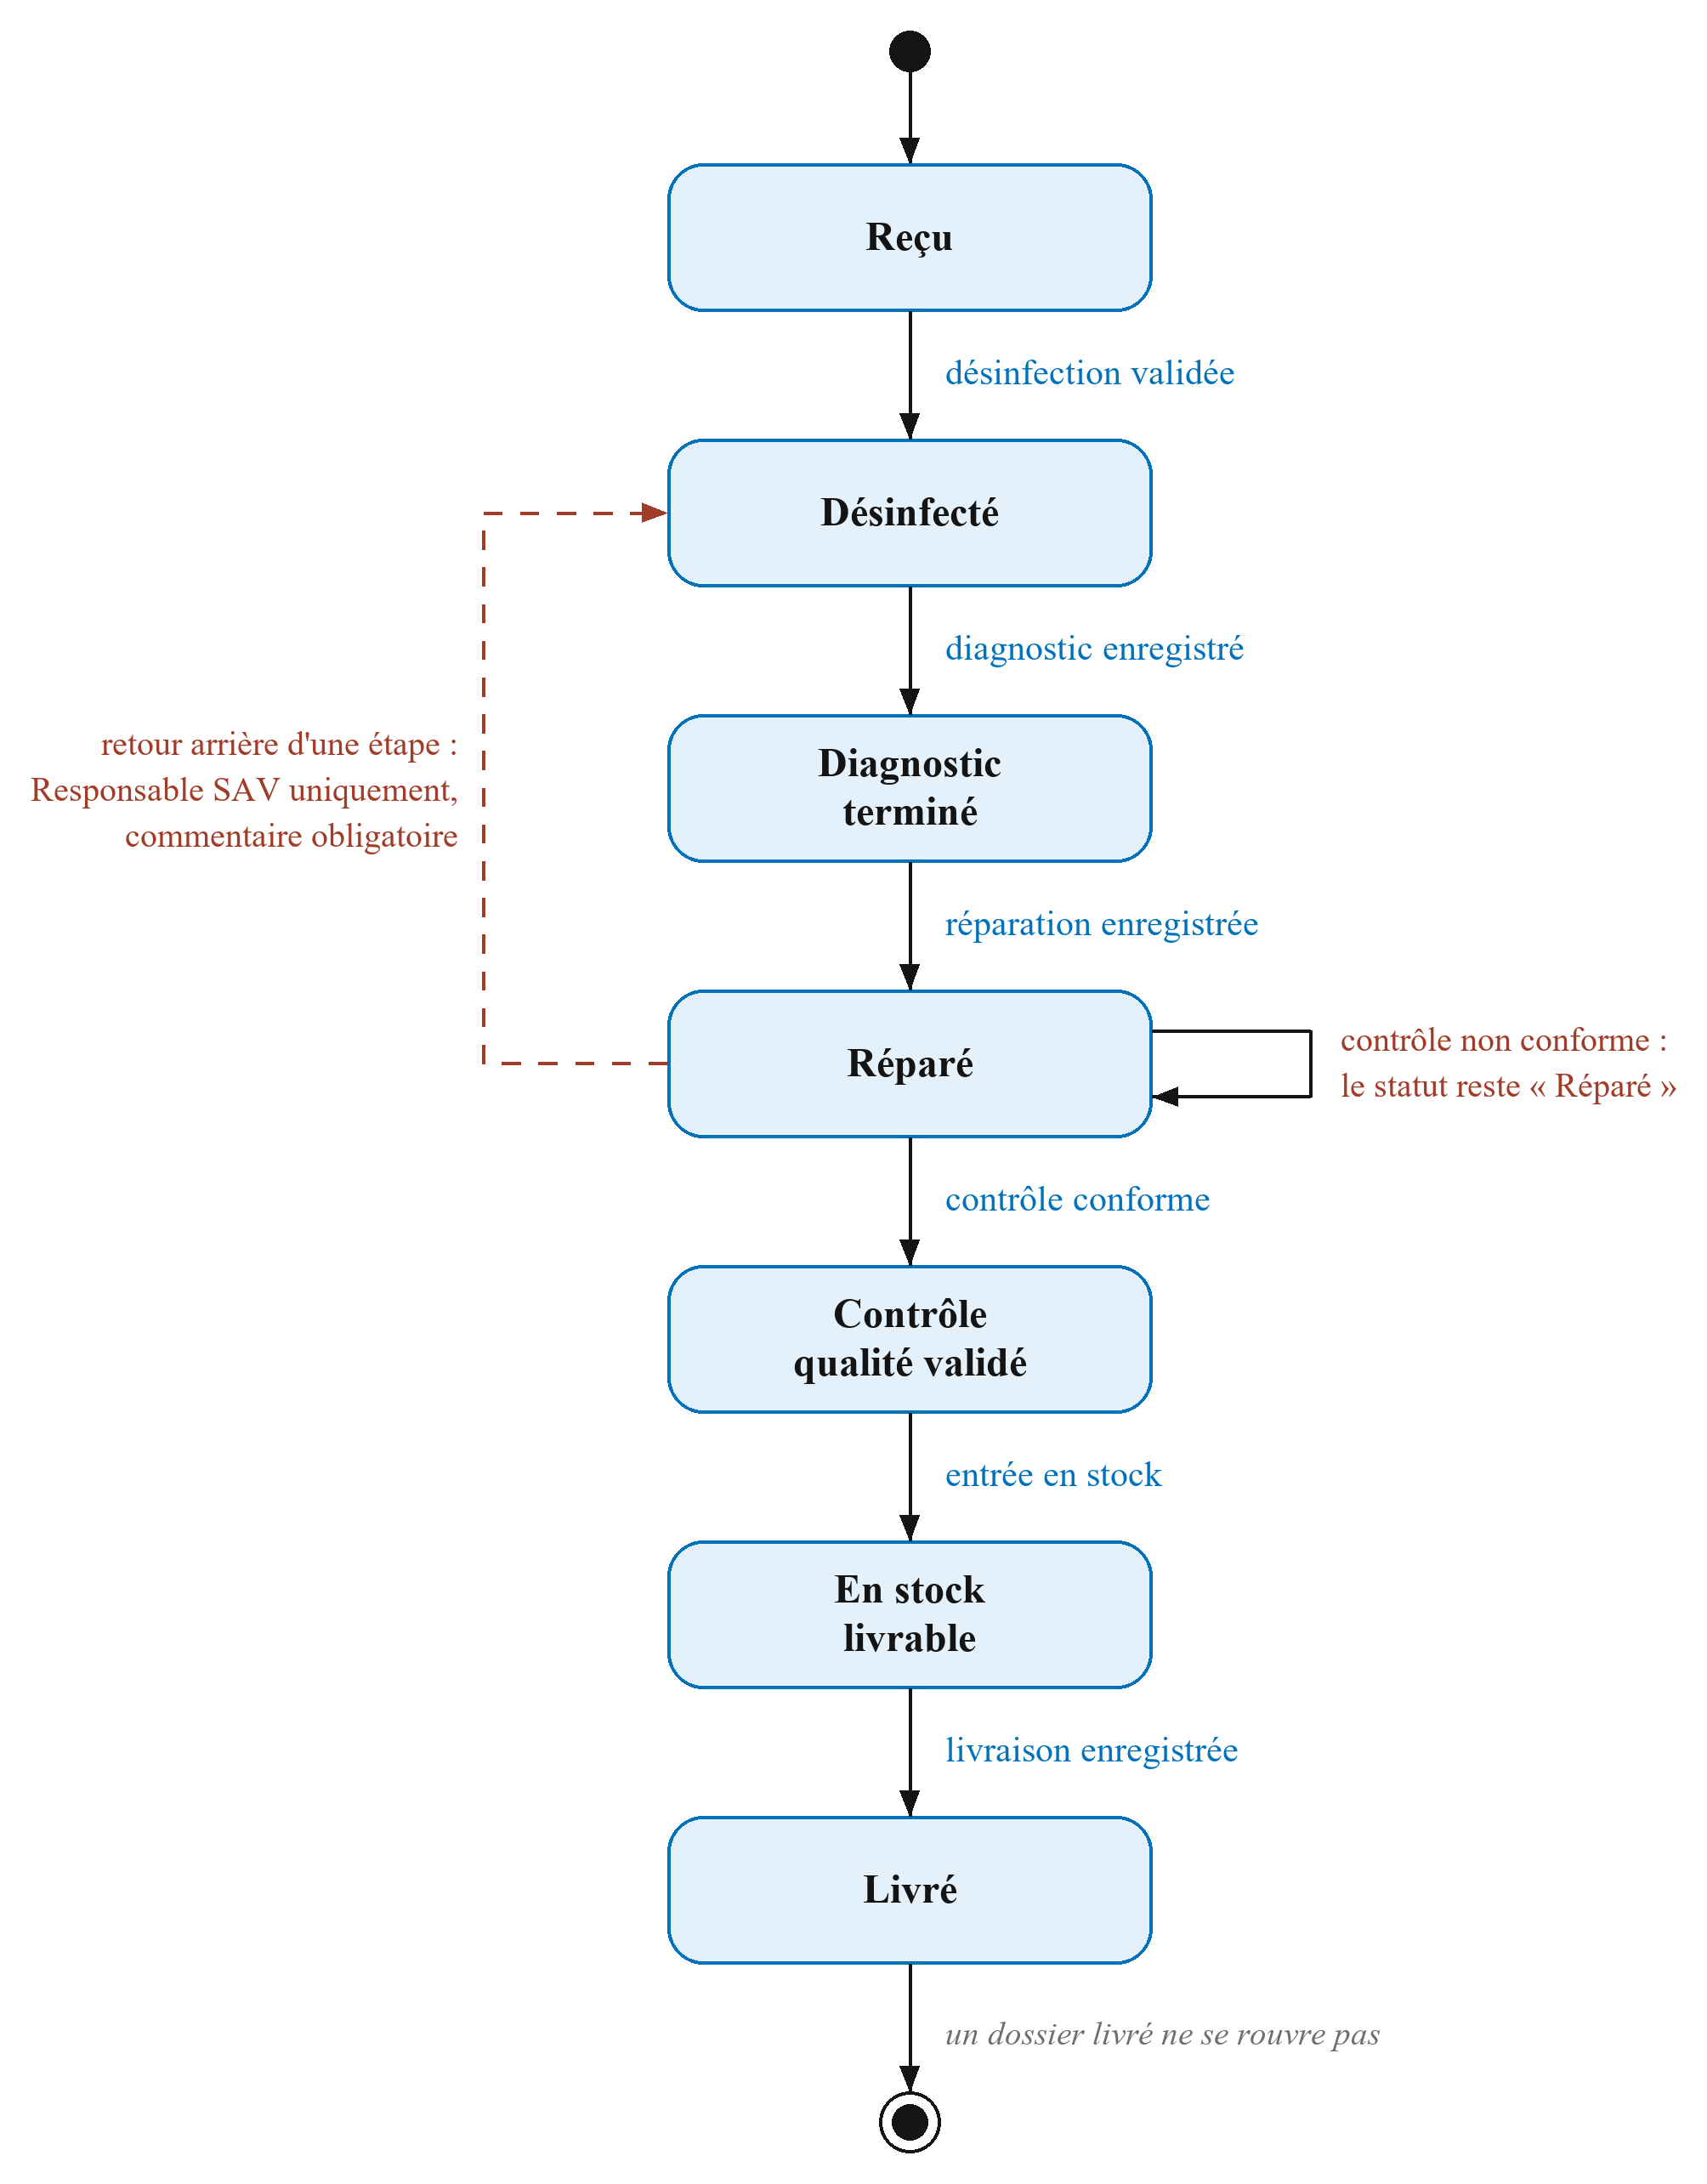
\includegraphics[width=15.5cm,height=18.5cm,keepaspectratio]{uml_etats.png}
\caption{Diagramme d'états d'un dossier SAV}
\end{figure}

\Needspace{14\baselineskip}

{\small\setstretch{1.05}\renewcommand{\arraystretch}{1.3}\arrayrulecolor{ALtexte}
\begin{longtable}{|>{\raggedright\arraybackslash}p{3.56cm}|>{\raggedright\arraybackslash}p{3.12cm}|>{\raggedright\arraybackslash}p{7.57cm}|}
\caption{Statuts du dossier SAV et prérequis}\\
\hline
\rowcolor{ALbleu} \sffamily\bfseries\color{white} Statut & \sffamily\bfseries\color{white} Étape validée & \sffamily\bfseries\color{white} Prérequis pour y accéder \\ \hline
\endfirsthead
\caption[]{Statuts du dossier SAV et prérequis (suite)}\\
\hline
\rowcolor{ALbleu} \sffamily\bfseries\color{white} Statut & \sffamily\bfseries\color{white} Étape validée & \sffamily\bfseries\color{white} Prérequis pour y accéder \\ \hline
\endhead
RECU & Réception & Appareil identifié par son numéro de série \\ \hline
\rowcolor{ALgris} DESINFECTE & Désinfection & Désinfection enregistrée et validée \\ \hline
DIAGNOSTIC\_\allowbreak{}TERMINE & Diagnostic & Diagnostic enregistré (pannes du type d'appareil) \\ \hline
\rowcolor{ALgris} REPARE & Réparation & Réparation enregistrée (début, fin, pièces) \\ \hline
QC\_\allowbreak{}VALIDE & Contrôle qualité & Dernier contrôle conforme sur les 7 points \\ \hline
\rowcolor{ALgris} EN\_\allowbreak{}STOCK & Entrée en stock & Emplacement renseigné \\ \hline
LIVRE & Livraison & Destinataire renseigné \\ \hline
\end{longtable}
}

\subsection{Règles métier}

\begin{itemize}
  \item un appareil physique possède \textbf{une seule fiche} (numéro de série normalisé) et peut avoir plusieurs retours ;
  \item un appareil ne peut avoir \textbf{qu'un seul dossier ouvert} à la fois (contrainte en base de données) ;
  \item aucun saut d'étape n'est possible ; le statut ne se modifie pas directement par l'API ;
  \item le \textbf{retour arrière} est réservé au Responsable SAV avec commentaire obligatoire, et un dossier livré ne se rouvre pas ;
  \item un contrôle qualité non conforme exige un commentaire, laisse le dossier à l'état \og{}réparé\fg{} et bloque la mise en stock ;
  \item le \textbf{risque biologique} est déduit du questionnaire : un statut \og{}inconnu\fg{} est traité comme un risque, par précaution ;
  \item les pannes d'un diagnostic doivent appartenir au type de l'appareil.
\end{itemize}

\subsection{Modèle de données}

Une décision de conception importante a été de \textbf{séparer l'appareil physique de ses retours}. La première version de la conception reposait sur une entité unique \og{}Machine\fg{} ; elle a évolué vers deux entités : l'\textbf{appareil} (fiche de vie durable, créée une seule fois) et le \textbf{dossier SAV} (un retour, avec ses étapes). Ainsi, un appareil qui revient plusieurs fois au service n'est jamais recréé.

Le modèle est présenté en deux diagrammes de classes : le premier montre le cœur (utilisateurs, appareils, retours et historique), le second les étapes rattachées à un dossier.

\begin{figure}[p]
\centering
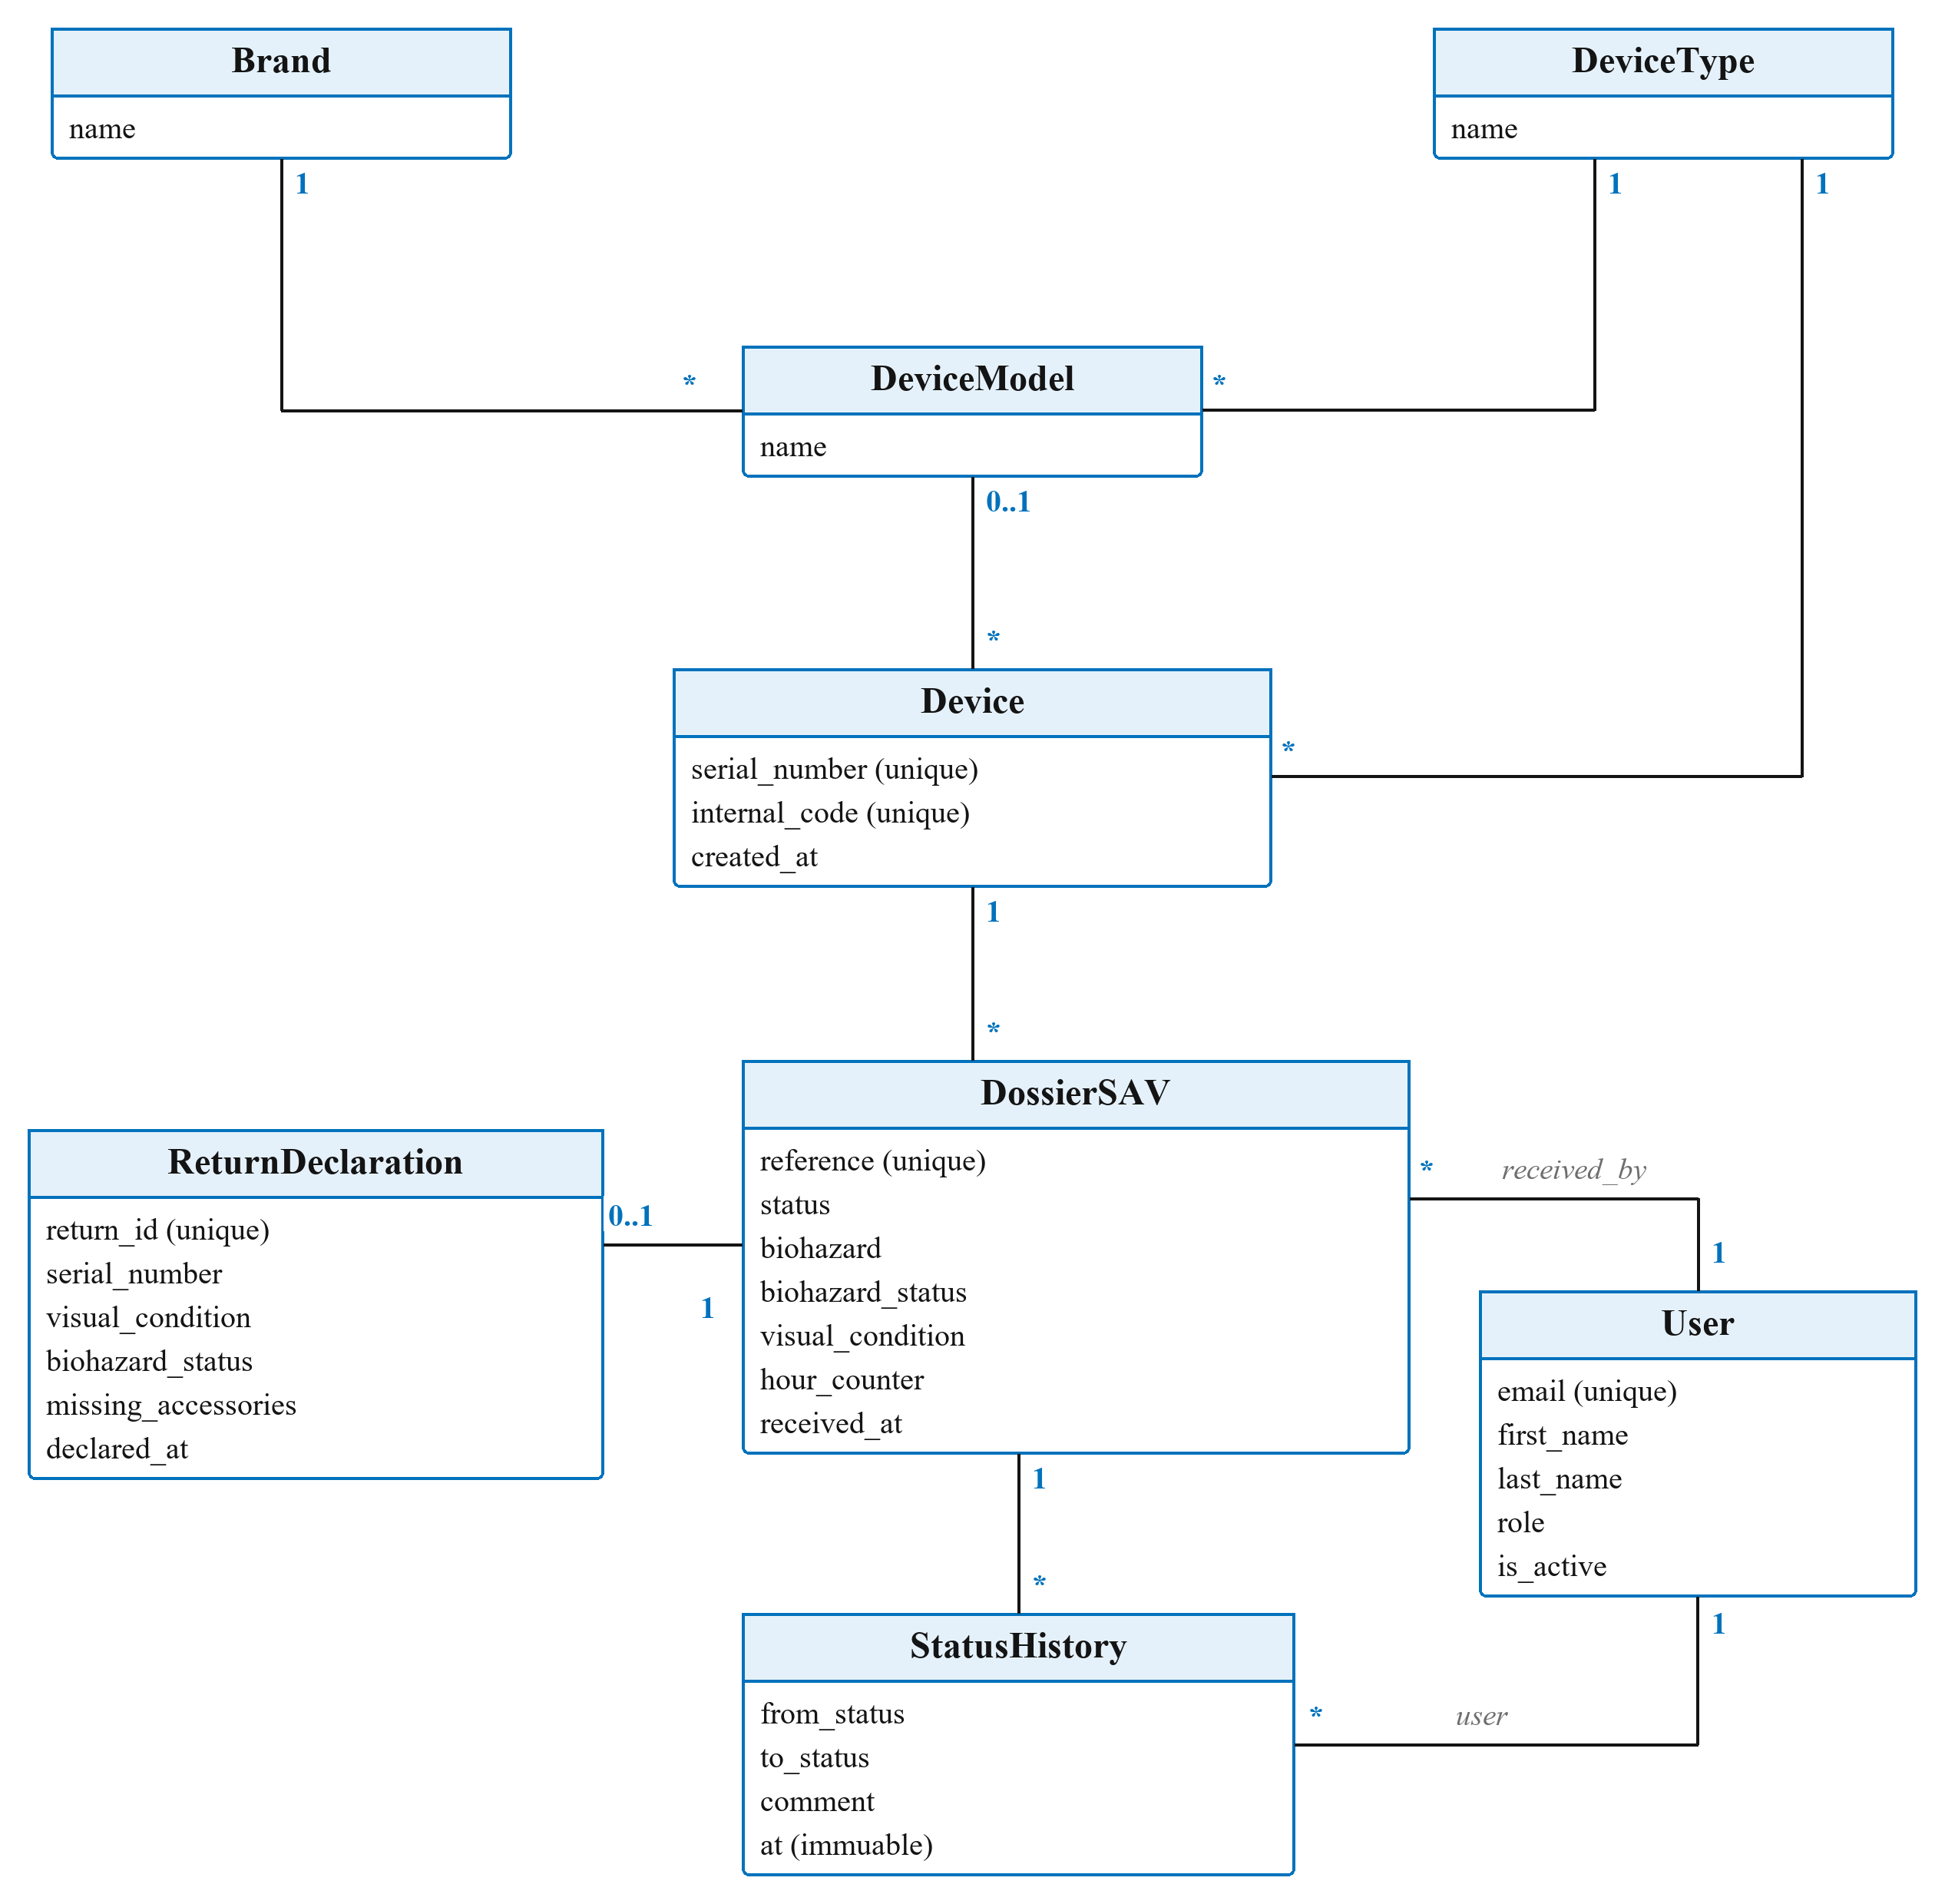
\includegraphics[width=15.5cm,height=18.5cm,keepaspectratio]{uml_classes_coeur.png}
\caption{Diagramme de classes : appareil, retour et historique}
\end{figure}

\begin{figure}[p]
\centering
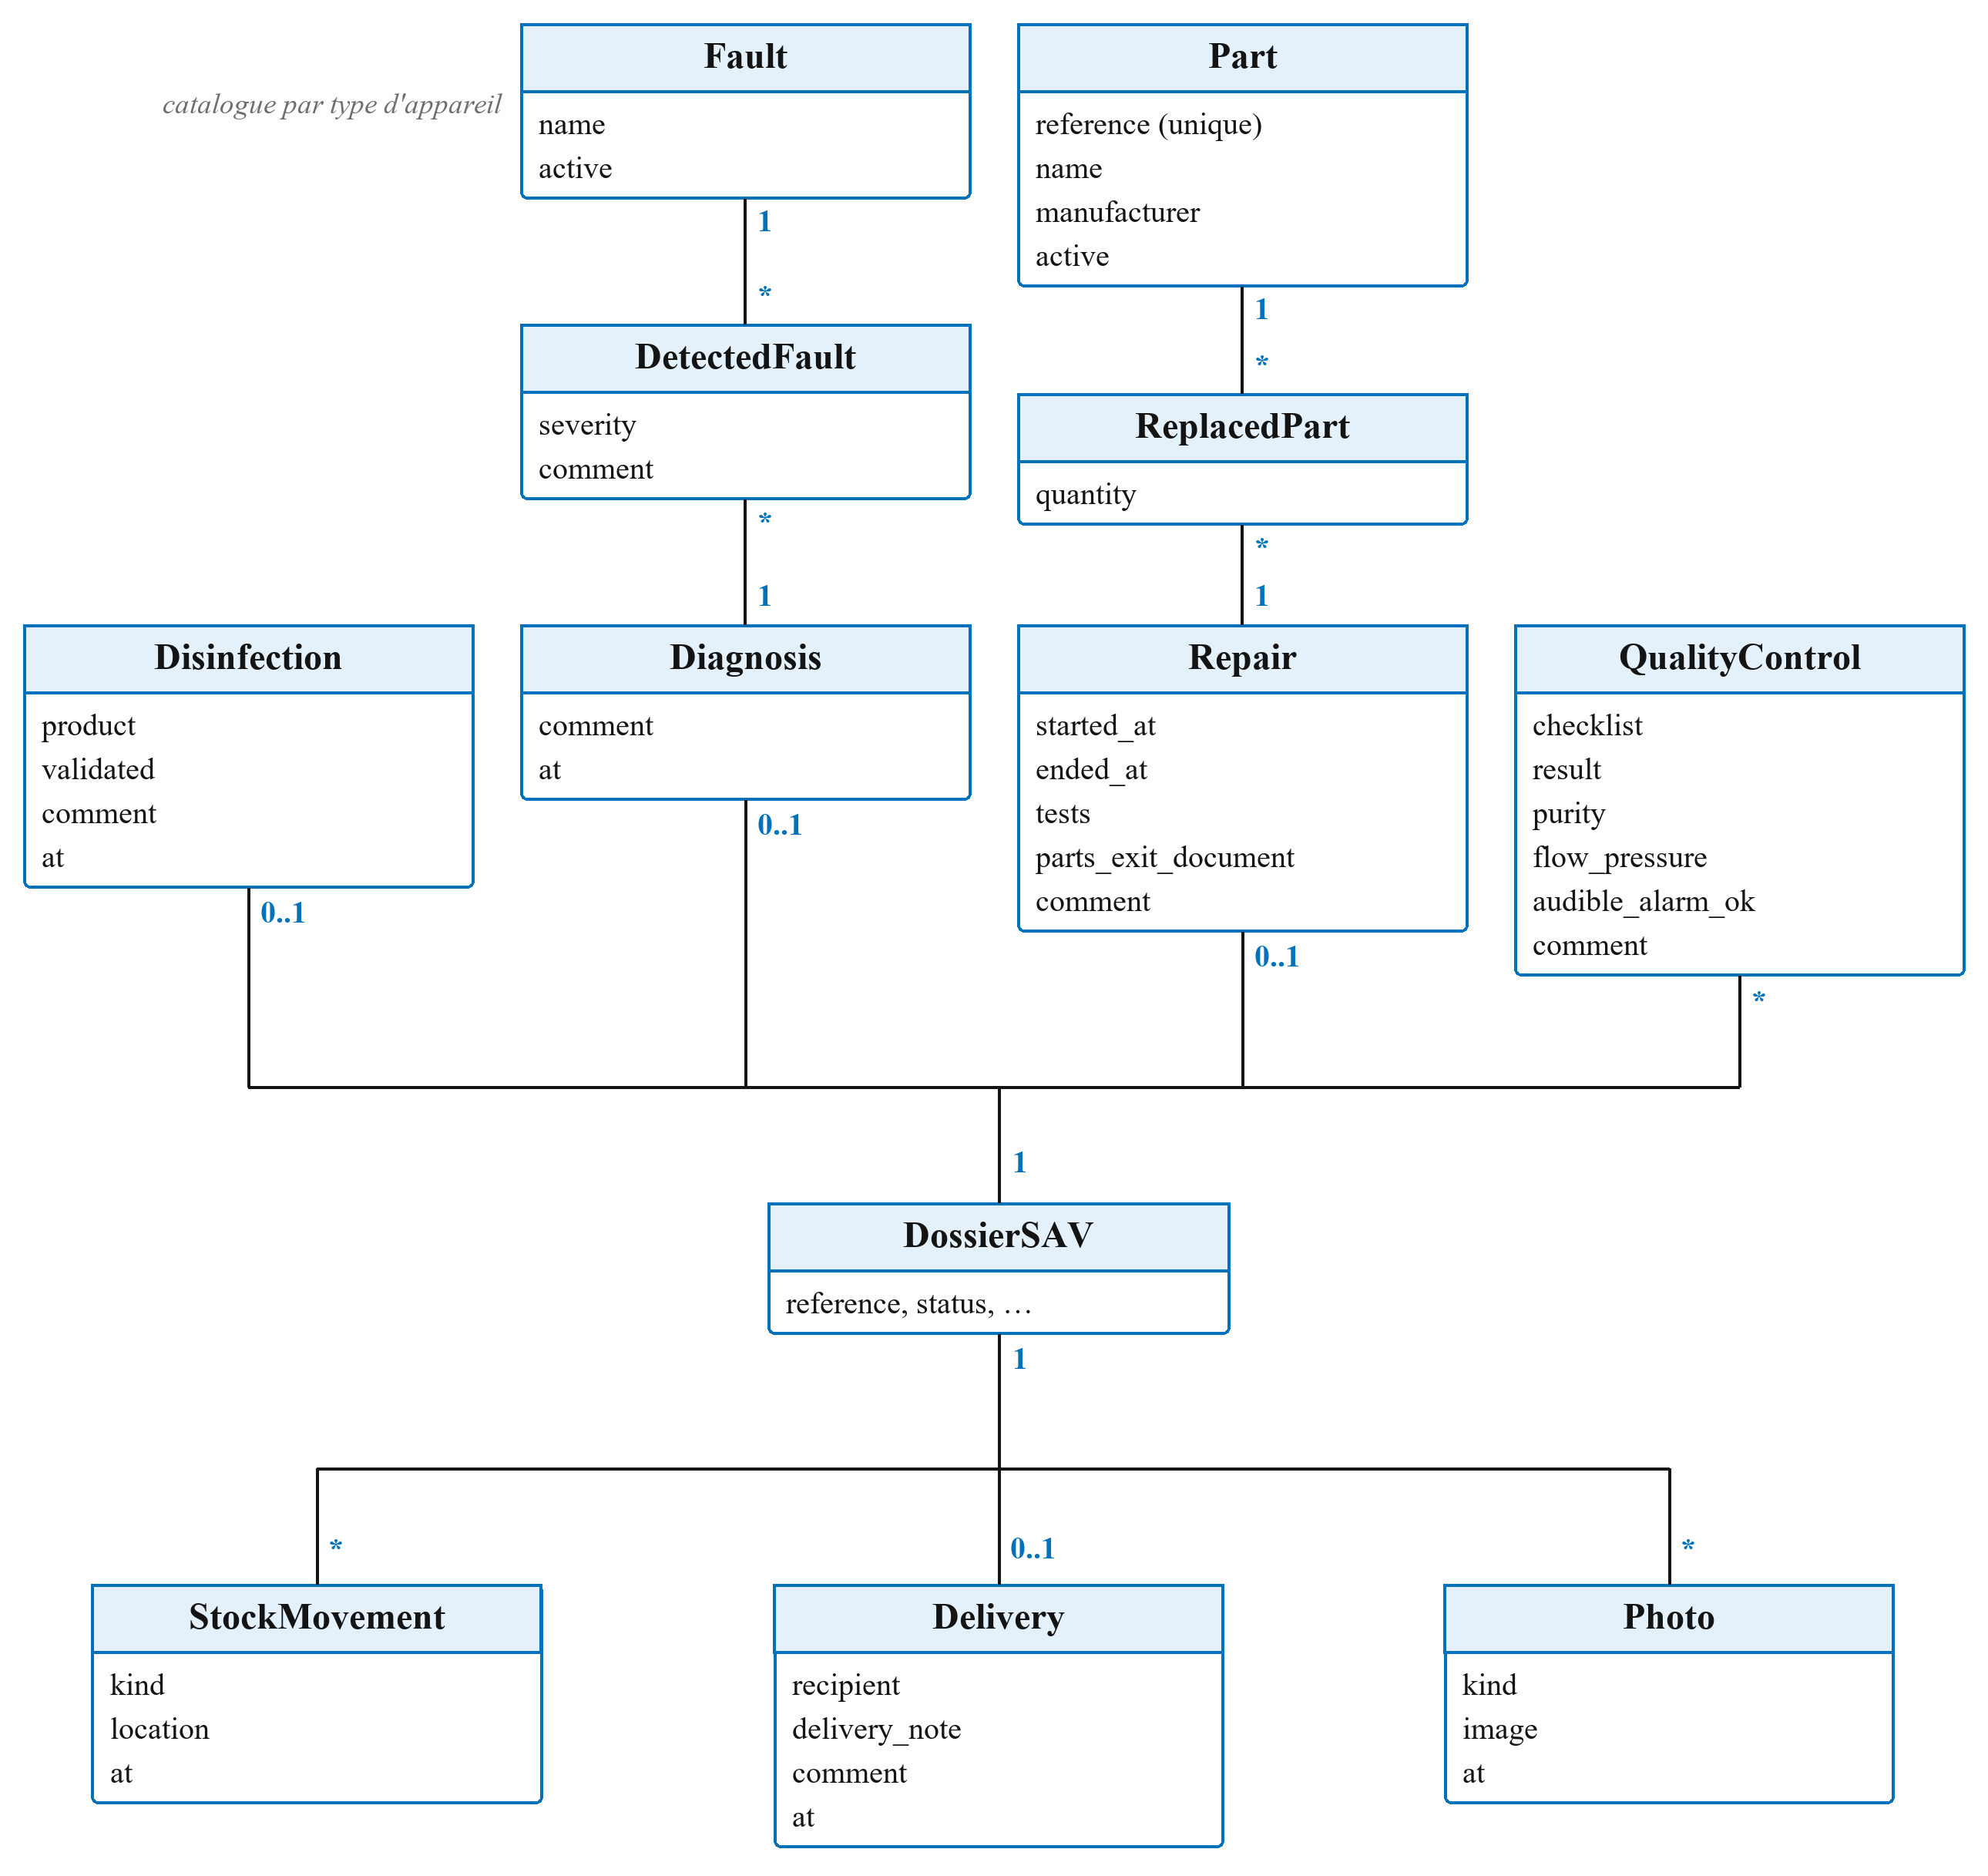
\includegraphics[width=15.5cm,height=18.5cm,keepaspectratio]{uml_classes_etapes.png}
\caption{Diagramme de classes : étapes rattachées au dossier SAV}
\end{figure}

Le modèle comprend 19 entités et 2 énumérations (annexe B), organisées autour de quatre groupes : utilisateurs, référentiel d'appareils (types, marques, modèles, appareils), dossier SAV et ses étapes, catalogues (pannes, pièces).

\subsection{Architecture}

L'application suit une architecture client / serveur en couches, fondée sur une API REST. Le frontend ne contient aucune règle métier : il appelle l'API, qui applique les règles dans une couche de services.

\begin{figure}[p]
\centering
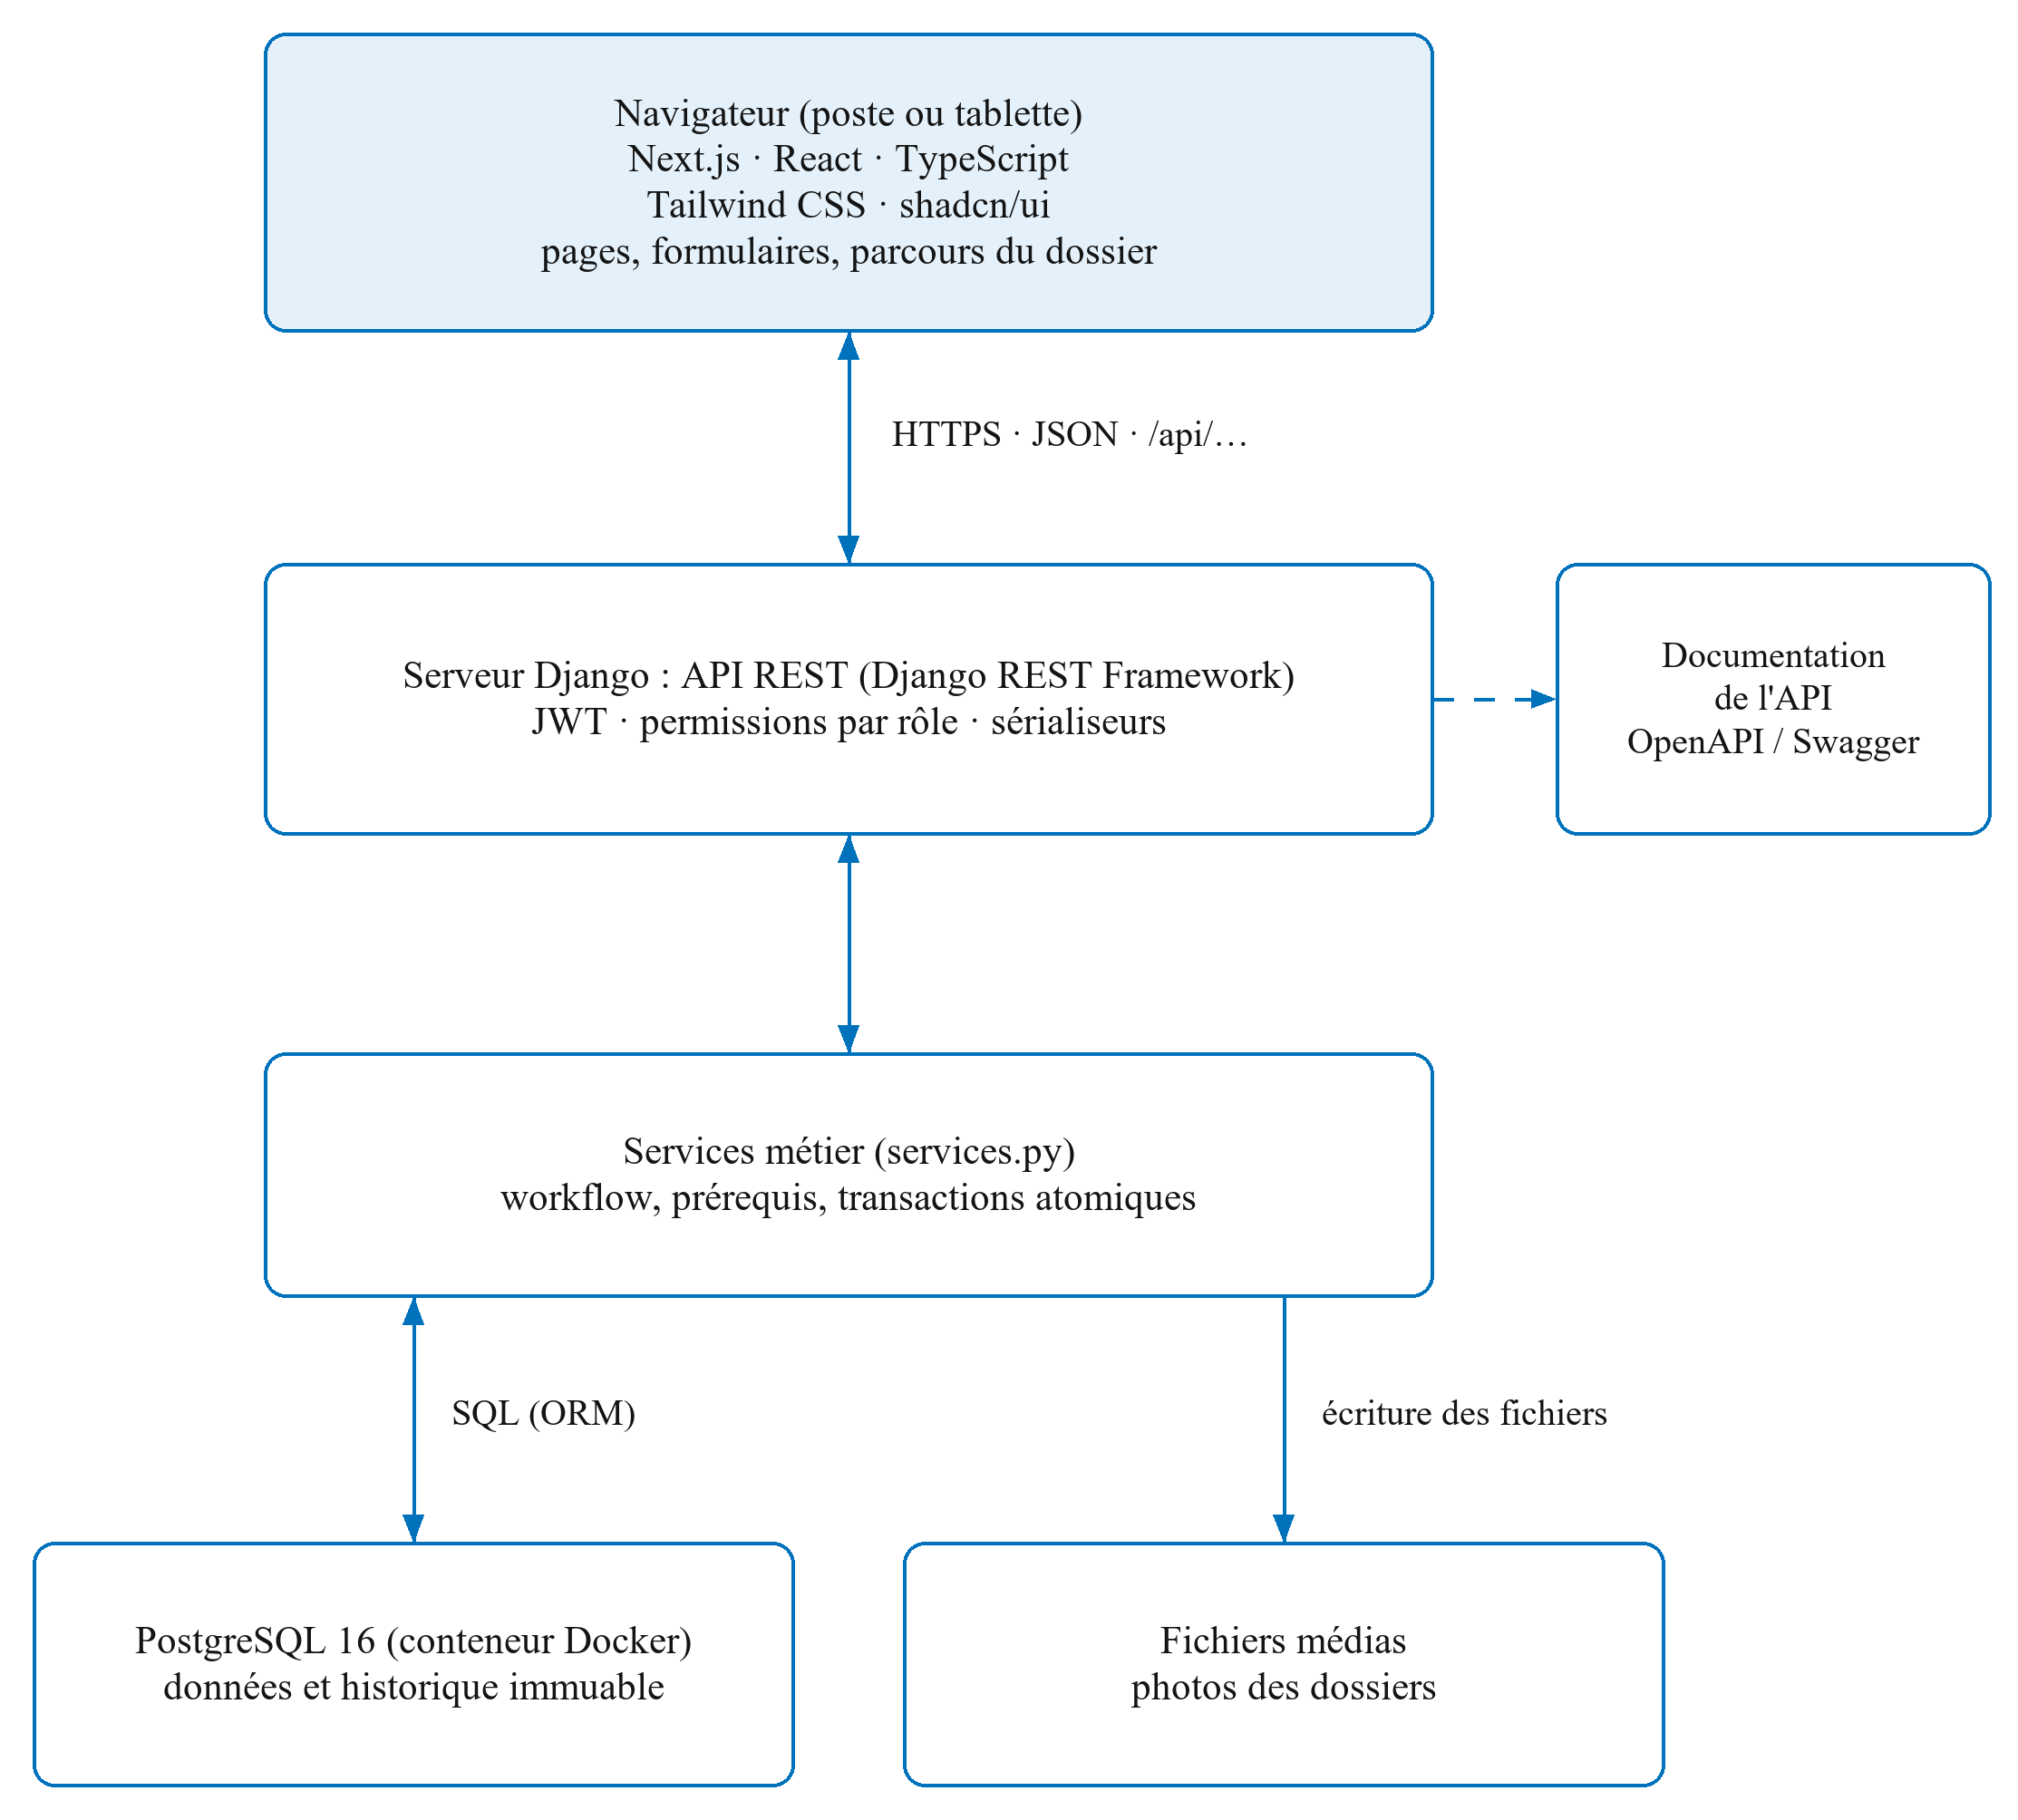
\includegraphics[width=15.5cm,height=18.5cm,keepaspectratio]{uml_architecture.png}
\caption{Architecture d'AirLiquide GMAO+}
\end{figure}

La conception initiale prévoyait une architecture modulaire orientée domaine, avec un module \texttt{maintenance} regroupant tout le cycle de vie, plus des modules \texttt{accounts}, \texttt{inventory}, \texttt{reports}, \texttt{dashboard} et \texttt{common}. Ce choix a été retenu. Le tableau suivant compare la cible initiale à ce qui a été réalisé.

\Needspace{14\baselineskip}

{\small\setstretch{1.05}\renewcommand{\arraystretch}{1.3}\arrayrulecolor{ALtexte}
\begin{longtable}{|>{\raggedright\arraybackslash}p{7.30cm}|>{\raggedright\arraybackslash}p{7.30cm}|}
\caption{Architecture cible et architecture réalisée}\\
\hline
\rowcolor{ALbleu} \sffamily\bfseries\color{white} Élément de l'architecture cible & \sffamily\bfseries\color{white} État dans l'application réalisée \\ \hline
\endfirsthead
\caption[]{Architecture cible et architecture réalisée (suite)}\\
\hline
\rowcolor{ALbleu} \sffamily\bfseries\color{white} Élément de l'architecture cible & \sffamily\bfseries\color{white} État dans l'application réalisée \\ \hline
\endhead
Modules \texttt{accounts}, \texttt{maintenance}, \texttt{inventory}, \texttt{dashboard}, \texttt{reports} & Réalisés ; \texttt{common} créé mais non utilisé \\ \hline
\rowcolor{ALgris} Services (règles métier hors des vues) & Réalisés : \texttt{maintenance/\allowbreak{}services.\allowbreak{}py} \\ \hline
Selectors et repositories & Non réalisés : jugés inutiles à cette taille de projet \\ \hline
\rowcolor{ALgris} Frontend web Next.js / TypeScript / Tailwind / shadcn/ui & Réalisé \\ \hline
Application mobile Flutter & Non réalisée (prévue comme extension) \\ \hline
\rowcolor{ALgris} Docker & Partiel : seule la base PostgreSQL est conteneurisée \\ \hline
Rapports PDF, notifications, QR code & Non réalisés (perspectives) \\ \hline
\end{longtable}
}

\subsection{Sécurité}

\begin{itemize}
  \item \textbf{Authentification JWT} : le jeton d'accès reste en mémoire dans le navigateur ; le jeton de rafraîchissement est placé dans un cookie \texttt{HttpOnly}, inaccessible au code JavaScript (protection contre le vol de jeton) ;
  \item \textbf{limitation du nombre de tentatives} de connexion (10 par minute) ;
  \item \textbf{permissions par rôle} appliquées côté serveur, quelles que soient les actions de l'interface ;
  \item \textbf{validation côté serveur} de toutes les entrées ; contrôle des photos (formats JPEG, PNG, WebP, taille maximale 5 Mo, vérification du contenu) ;
  \item \textbf{exports CSV} protégés contre l'injection de formules dans les tableurs ;
  \item \textbf{secrets} (clé, mots de passe de base) hors du dépôt, dans un fichier d'environnement non versionné.
\end{itemize}

Le diagramme de séquence suivant détaille le cycle d'authentification : connexion, conservation du jeton d'accès en mémoire et renouvellement grâce au cookie.

\begin{figure}[p]
\centering
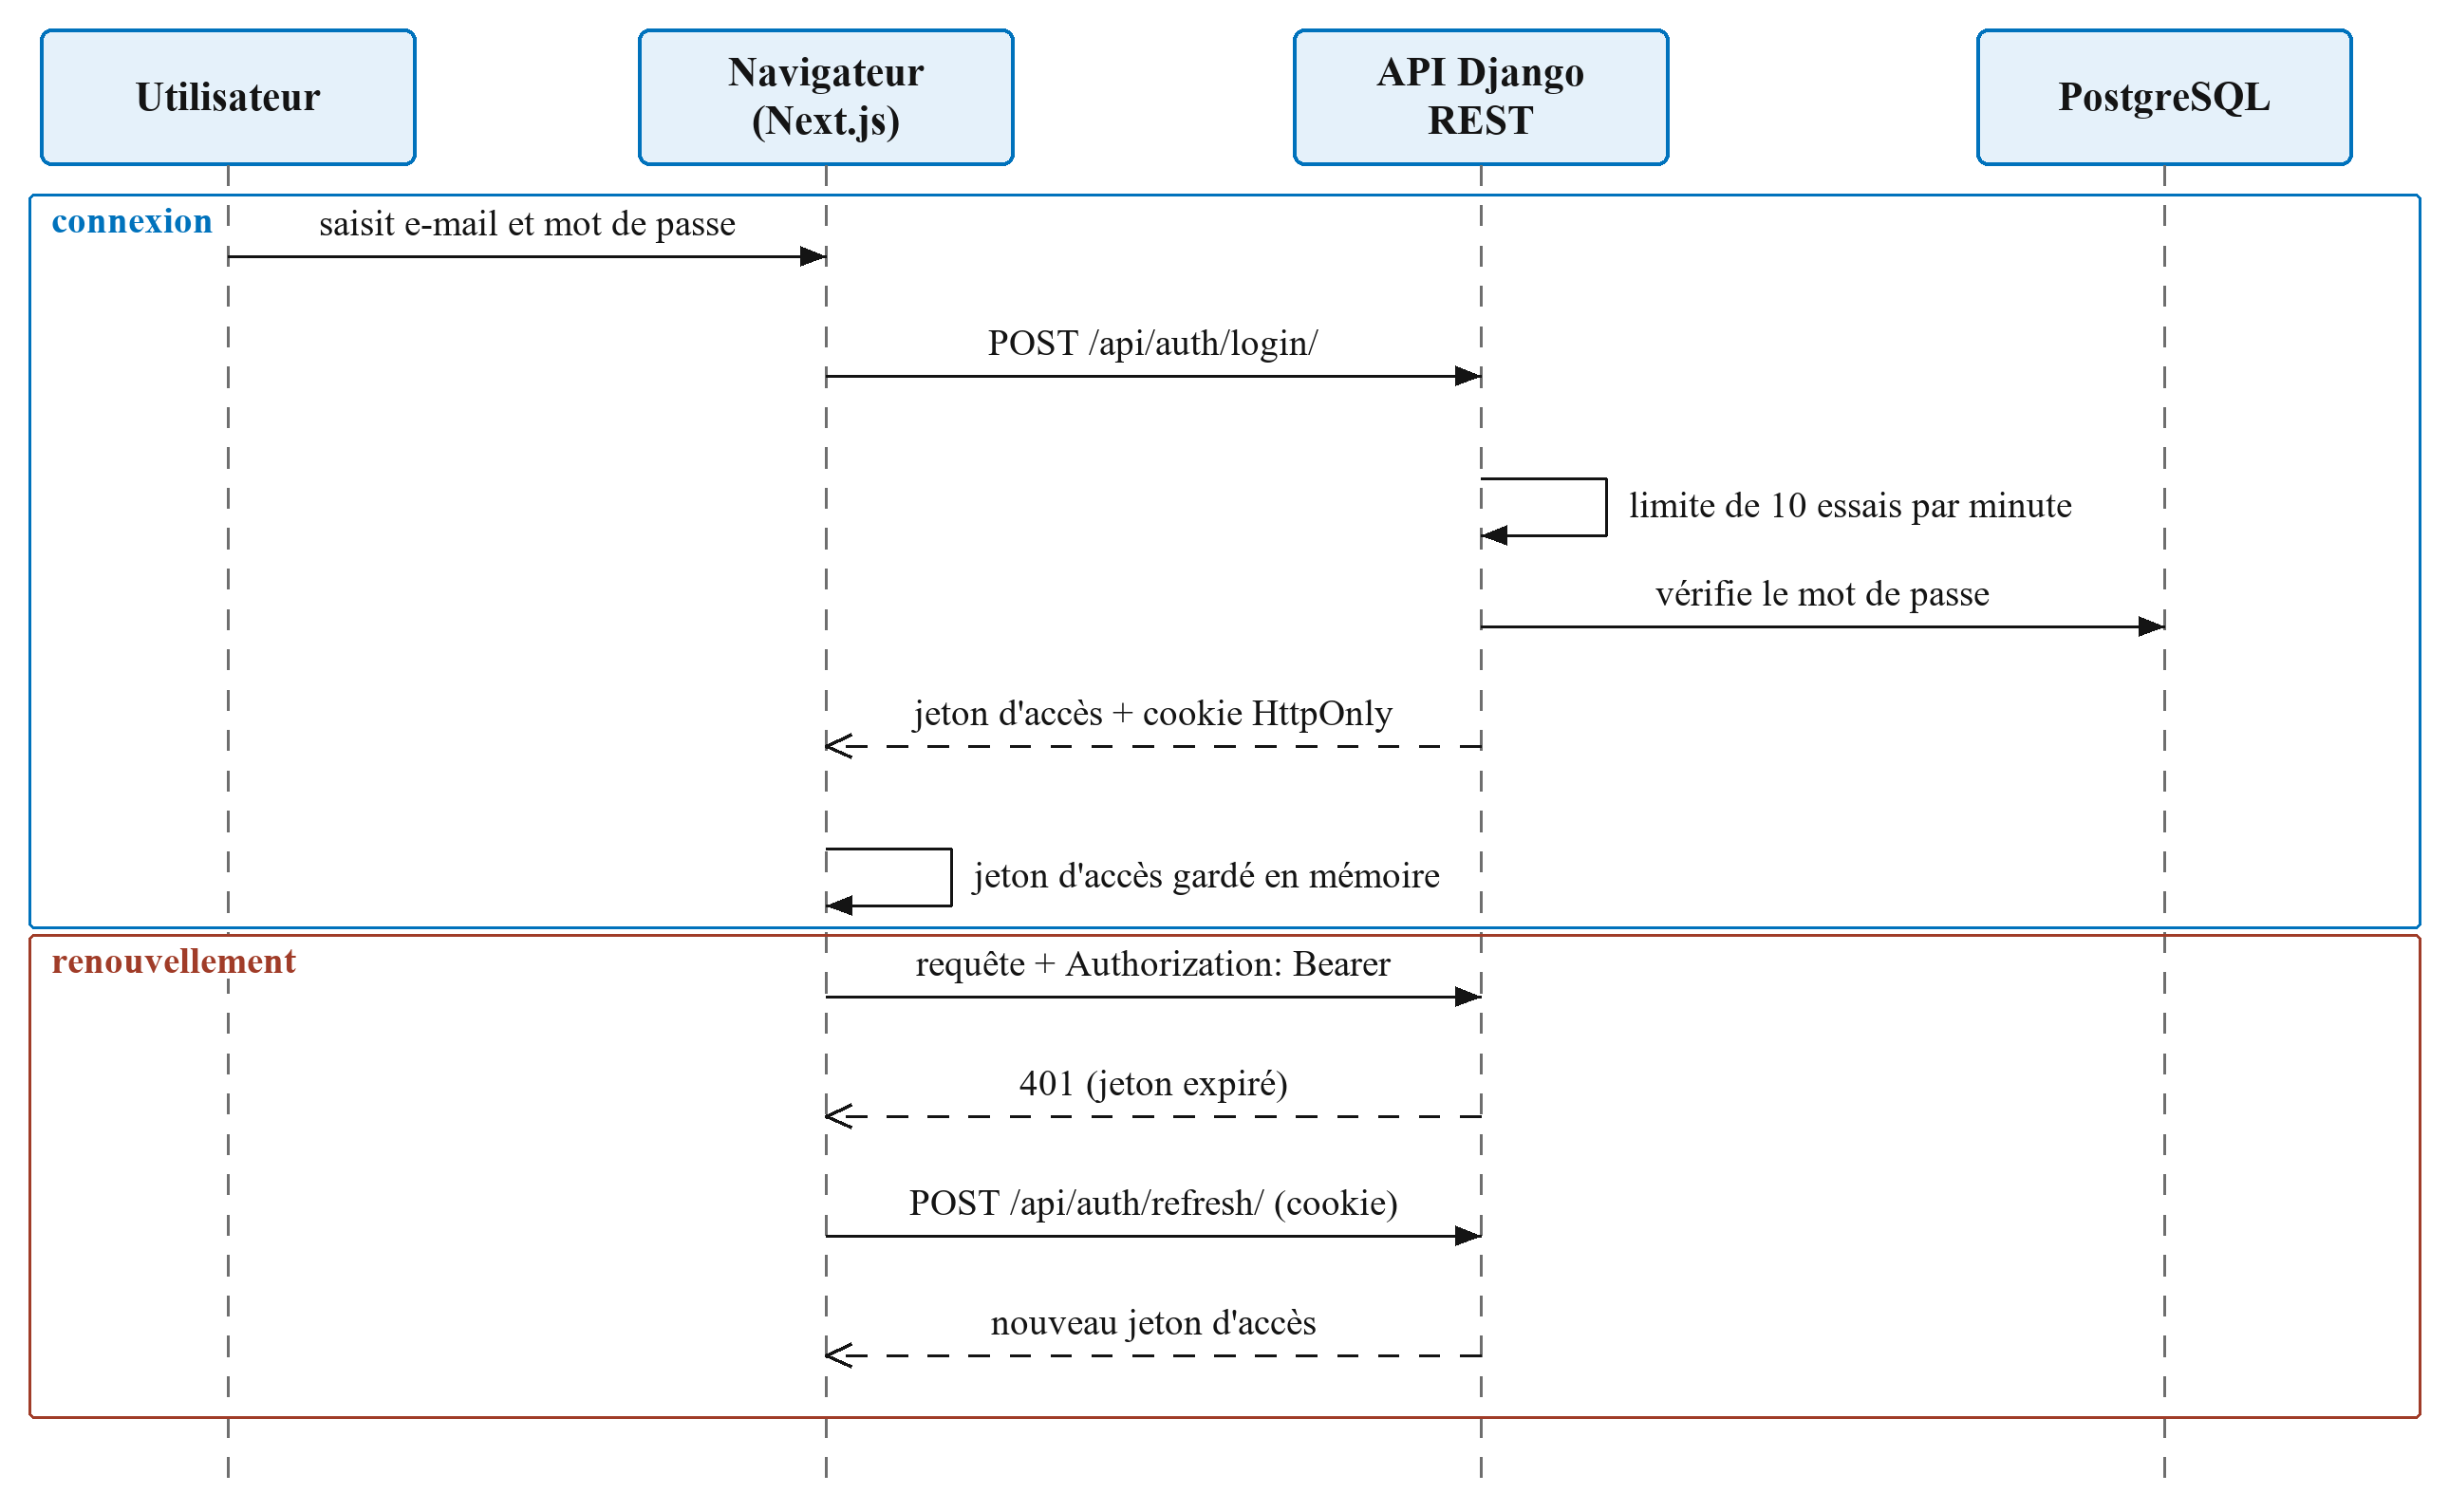
\includegraphics[width=15.5cm,height=18.5cm,keepaspectratio]{uml_sequence_auth.png}
\caption{Diagramme de séquence : authentification et renouvellement du jeton}
\end{figure}

\section{Réalisation}

\Needspace{15\baselineskip}
\subsection{Environnement technique}

{\small\setstretch{1.05}\renewcommand{\arraystretch}{1.3}\arrayrulecolor{ALtexte}
\begin{longtable}{|>{\raggedright\arraybackslash}p{3.20cm}|>{\raggedright\arraybackslash}p{11.41cm}|}
\caption{Environnement technique (versions relevées dans les fichiers de dépendances)}\\
\hline
\rowcolor{ALbleu} \sffamily\bfseries\color{white} Couche & \sffamily\bfseries\color{white} Technologies et versions \\ \hline
\endfirsthead
\caption[]{Environnement technique (versions relevées dans les fichiers de dépendances) (suite)}\\
\hline
\rowcolor{ALbleu} \sffamily\bfseries\color{white} Couche & \sffamily\bfseries\color{white} Technologies et versions \\ \hline
\endhead
Backend & Python 3.10, Django 5.2.16, Django REST Framework 3.17.1, SimpleJWT 5.5.1, drf-spectacular 0.30.0, django-cors-headers 4.9.0, Pillow 12.3.0 \\ \hline
\rowcolor{ALgris} Base de données & PostgreSQL 16 (conteneur Docker) ; SQLite en repli pour le développement \\ \hline
Frontend & Next.js 16.4.3, React 19.3.0, TypeScript 5, Tailwind CSS 4, shadcn/ui, lucide-react, sonner \\ \hline
\rowcolor{ALgris} Documentation API & OpenAPI / Swagger généré automatiquement (\texttt{/\allowbreak{}api/\allowbreak{}docs/\allowbreak{}}) \\ \hline
Outils & Git et GitHub, Docker Compose, Chrome et outils de développement \\ \hline
\end{longtable}
}

\subsection{Le backend}

Le backend est organisé en applications Django. Les \textbf{vues} reçoivent la requête et délèguent ; les \textbf{sérialiseurs} valident les entrées ; les \textbf{services} (\texttt{maintenance/\allowbreak{}services.\allowbreak{}py}) exécutent les règles métier dans des transactions atomiques : réception, désinfection, diagnostic, réparation, contrôle qualité, entrée en stock, livraison et changement de statut. Chaque service verrouille le dossier, vérifie le statut attendu, enregistre l'étape, fait avancer le statut et écrit l'historique en une seule opération.

L'API expose des points d'accès REST documentés (annexe A). Les actions de workflow sont de simples \texttt{POST} sur le dossier (par exemple \texttt{/\allowbreak{}api/\allowbreak{}dossiers/\allowbreak{}\{id\}/\allowbreak{}quality-\allowbreak{}control/\allowbreak{}}), ce qui rend l'enregistrement d'une étape et le changement de statut indissociables.

\begin{figure}[p]
\centering
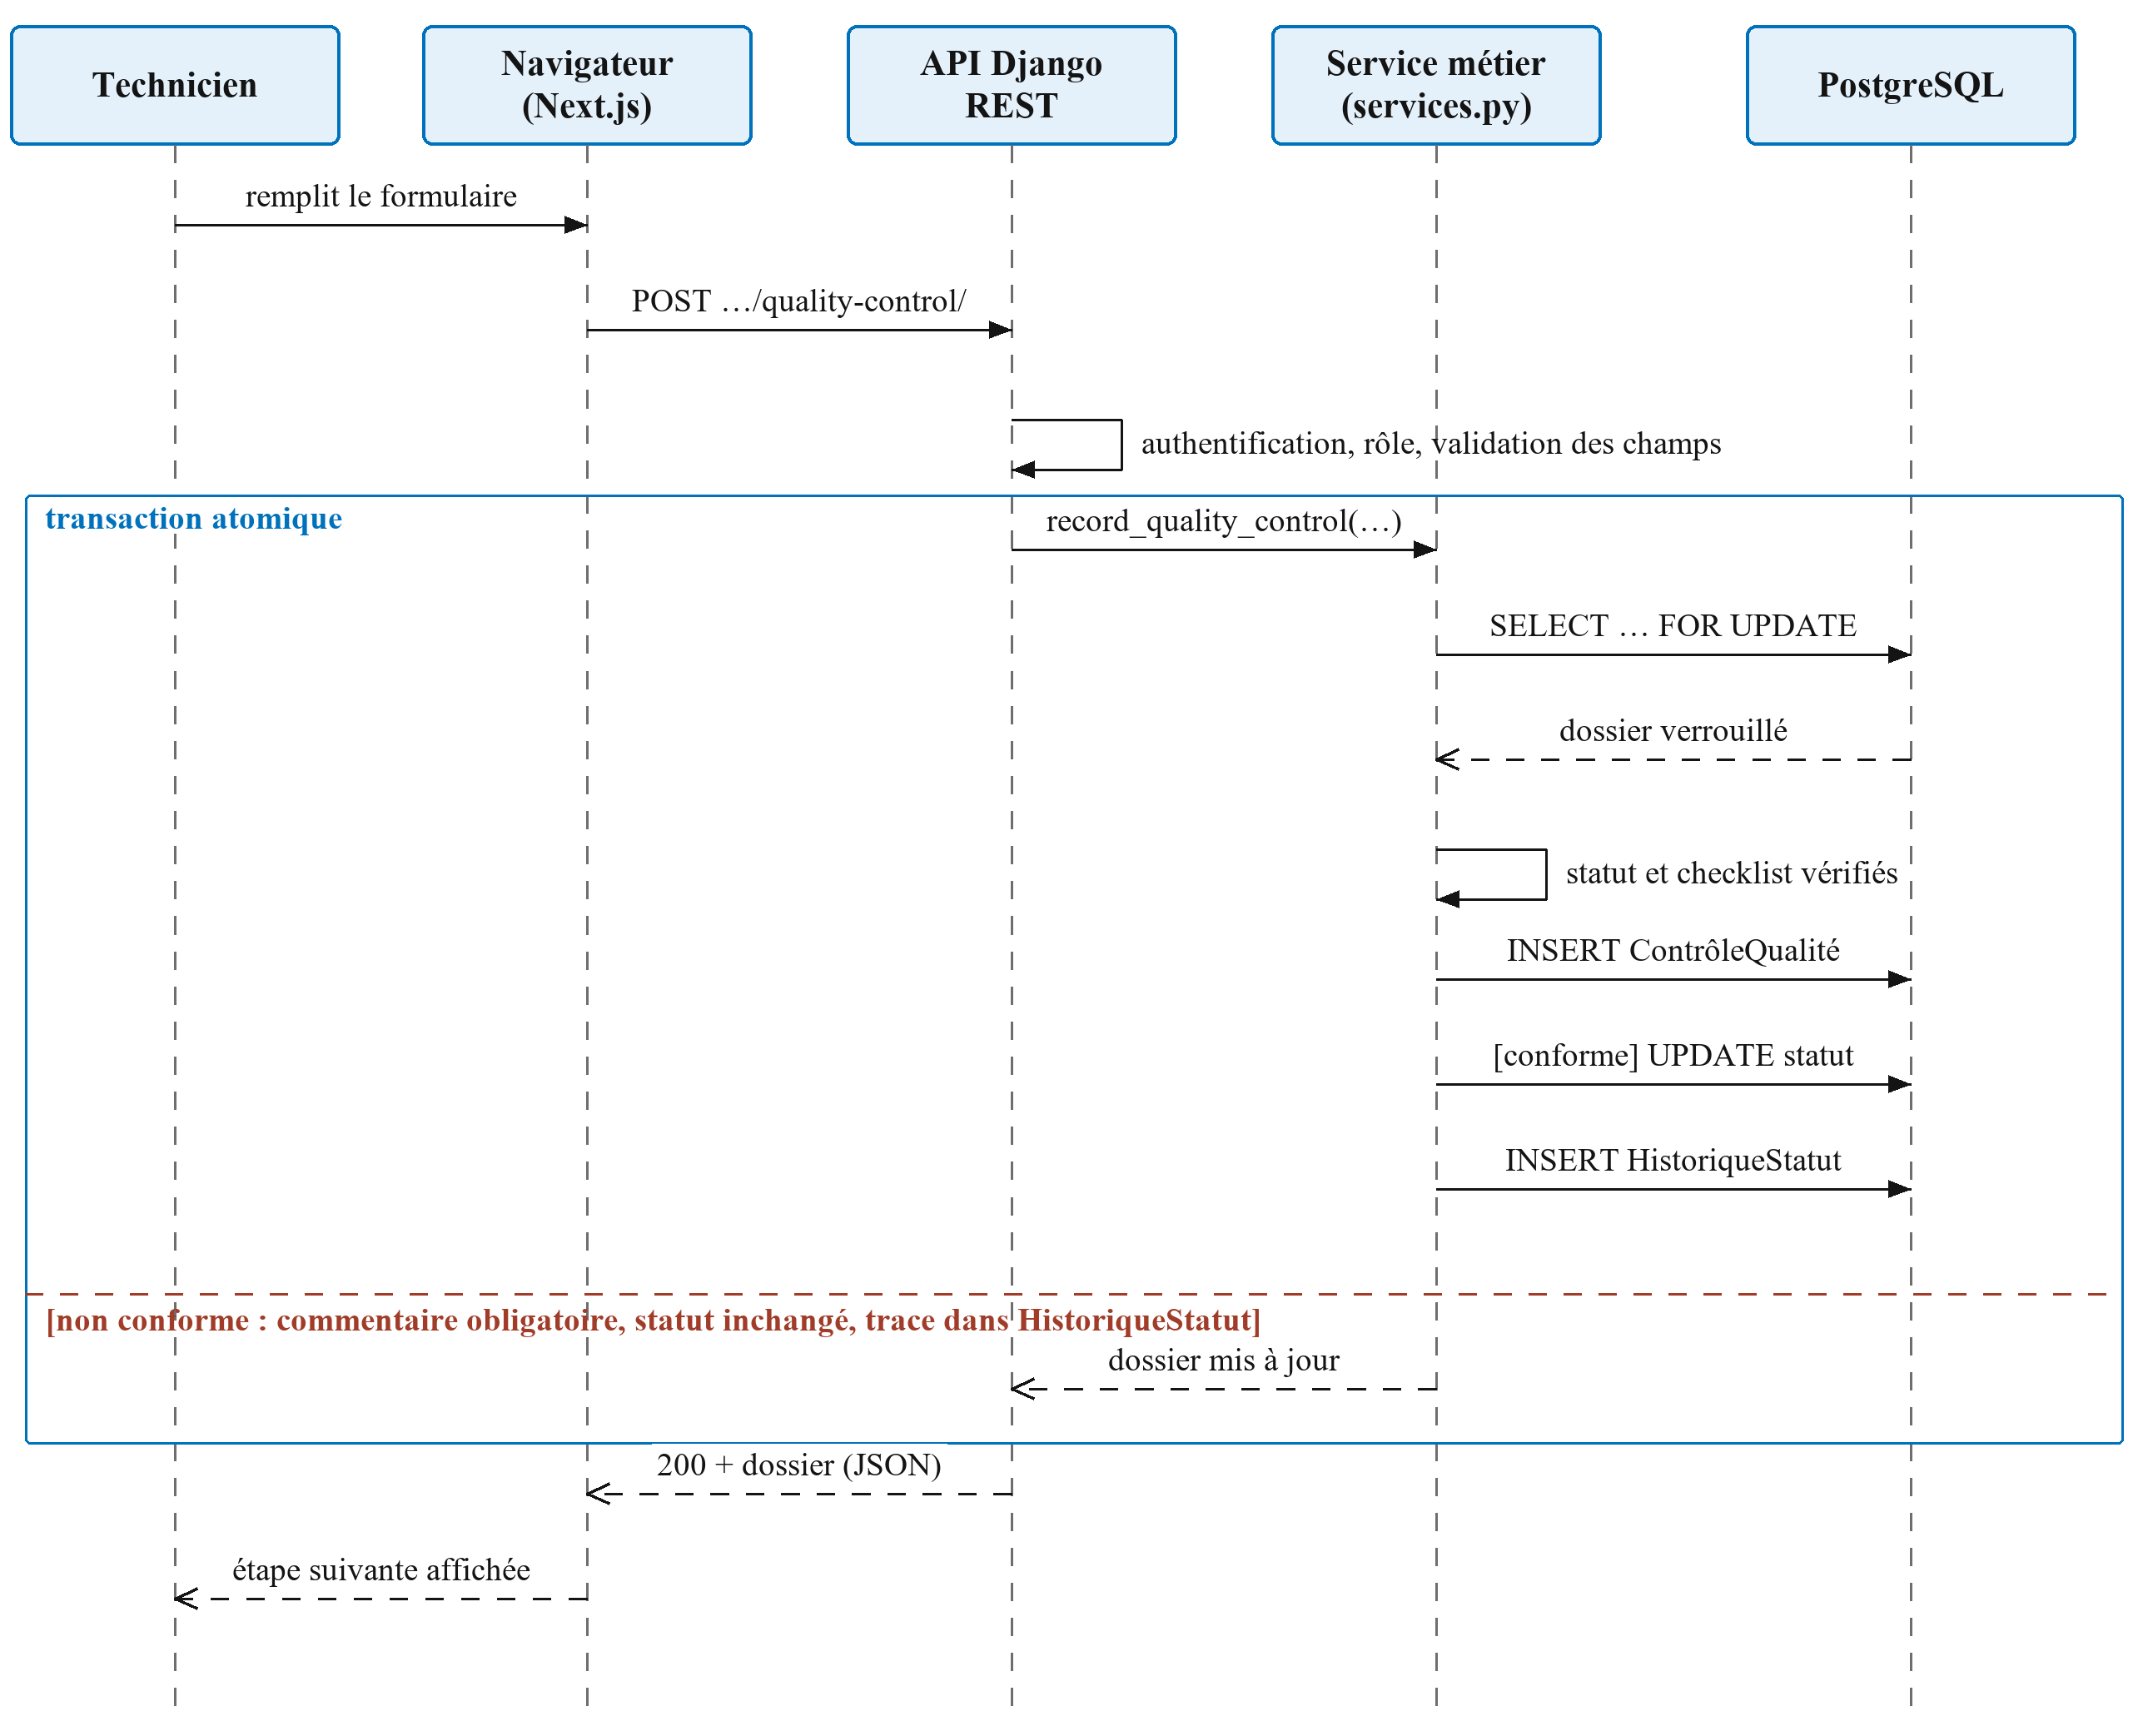
\includegraphics[width=15.5cm,height=18.5cm,keepaspectratio]{uml_sequence_etape.png}
\caption{Diagramme de séquence : enregistrement d'une étape (contrôle qualité)}
\end{figure}

\subsection{Le questionnaire de retour}

Le questionnaire en ligne existant a été intégré à l'application sous la forme d'une \textbf{annonce de retour} : avant l'arrivée de l'appareil, un utilisateur saisit le numéro de série, l'état visuel, les accessoires manquants, l'identifiant de retour et le statut biologique. À l'arrivée, le technicien choisit le retour annoncé dans l'écran de réception : les réponses sont reprises, le numéro de série est verrouillé et l'annonce est rattachée au dossier. Une annonce ne peut être réceptionnée qu'une seule fois.

\begin{figure}[!htb]
\centering
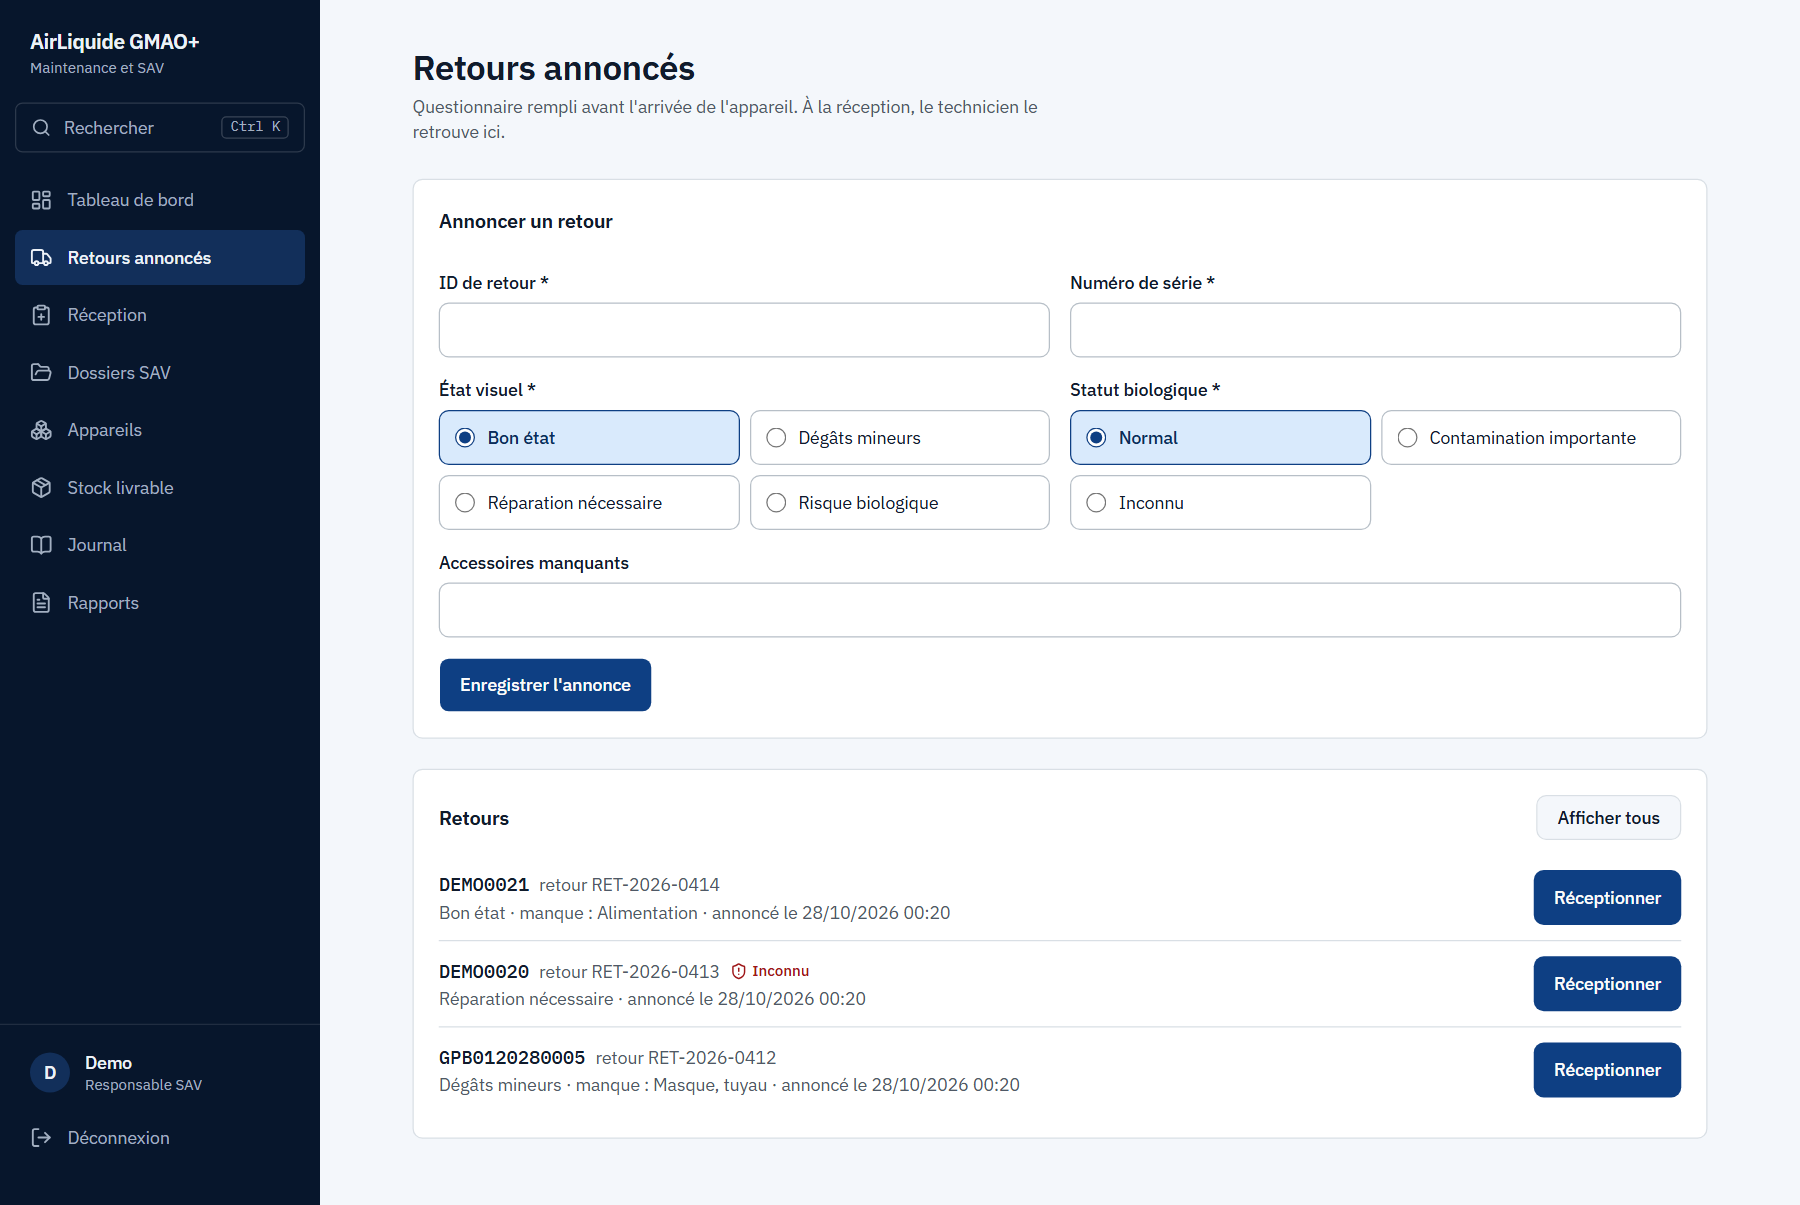
\includegraphics[width=15.0cm,height=17.5cm,keepaspectratio]{cap_retours.png}
\caption{Écran des retours annoncés (données de démonstration)}
\end{figure}

\begin{figure}[!htb]
\centering
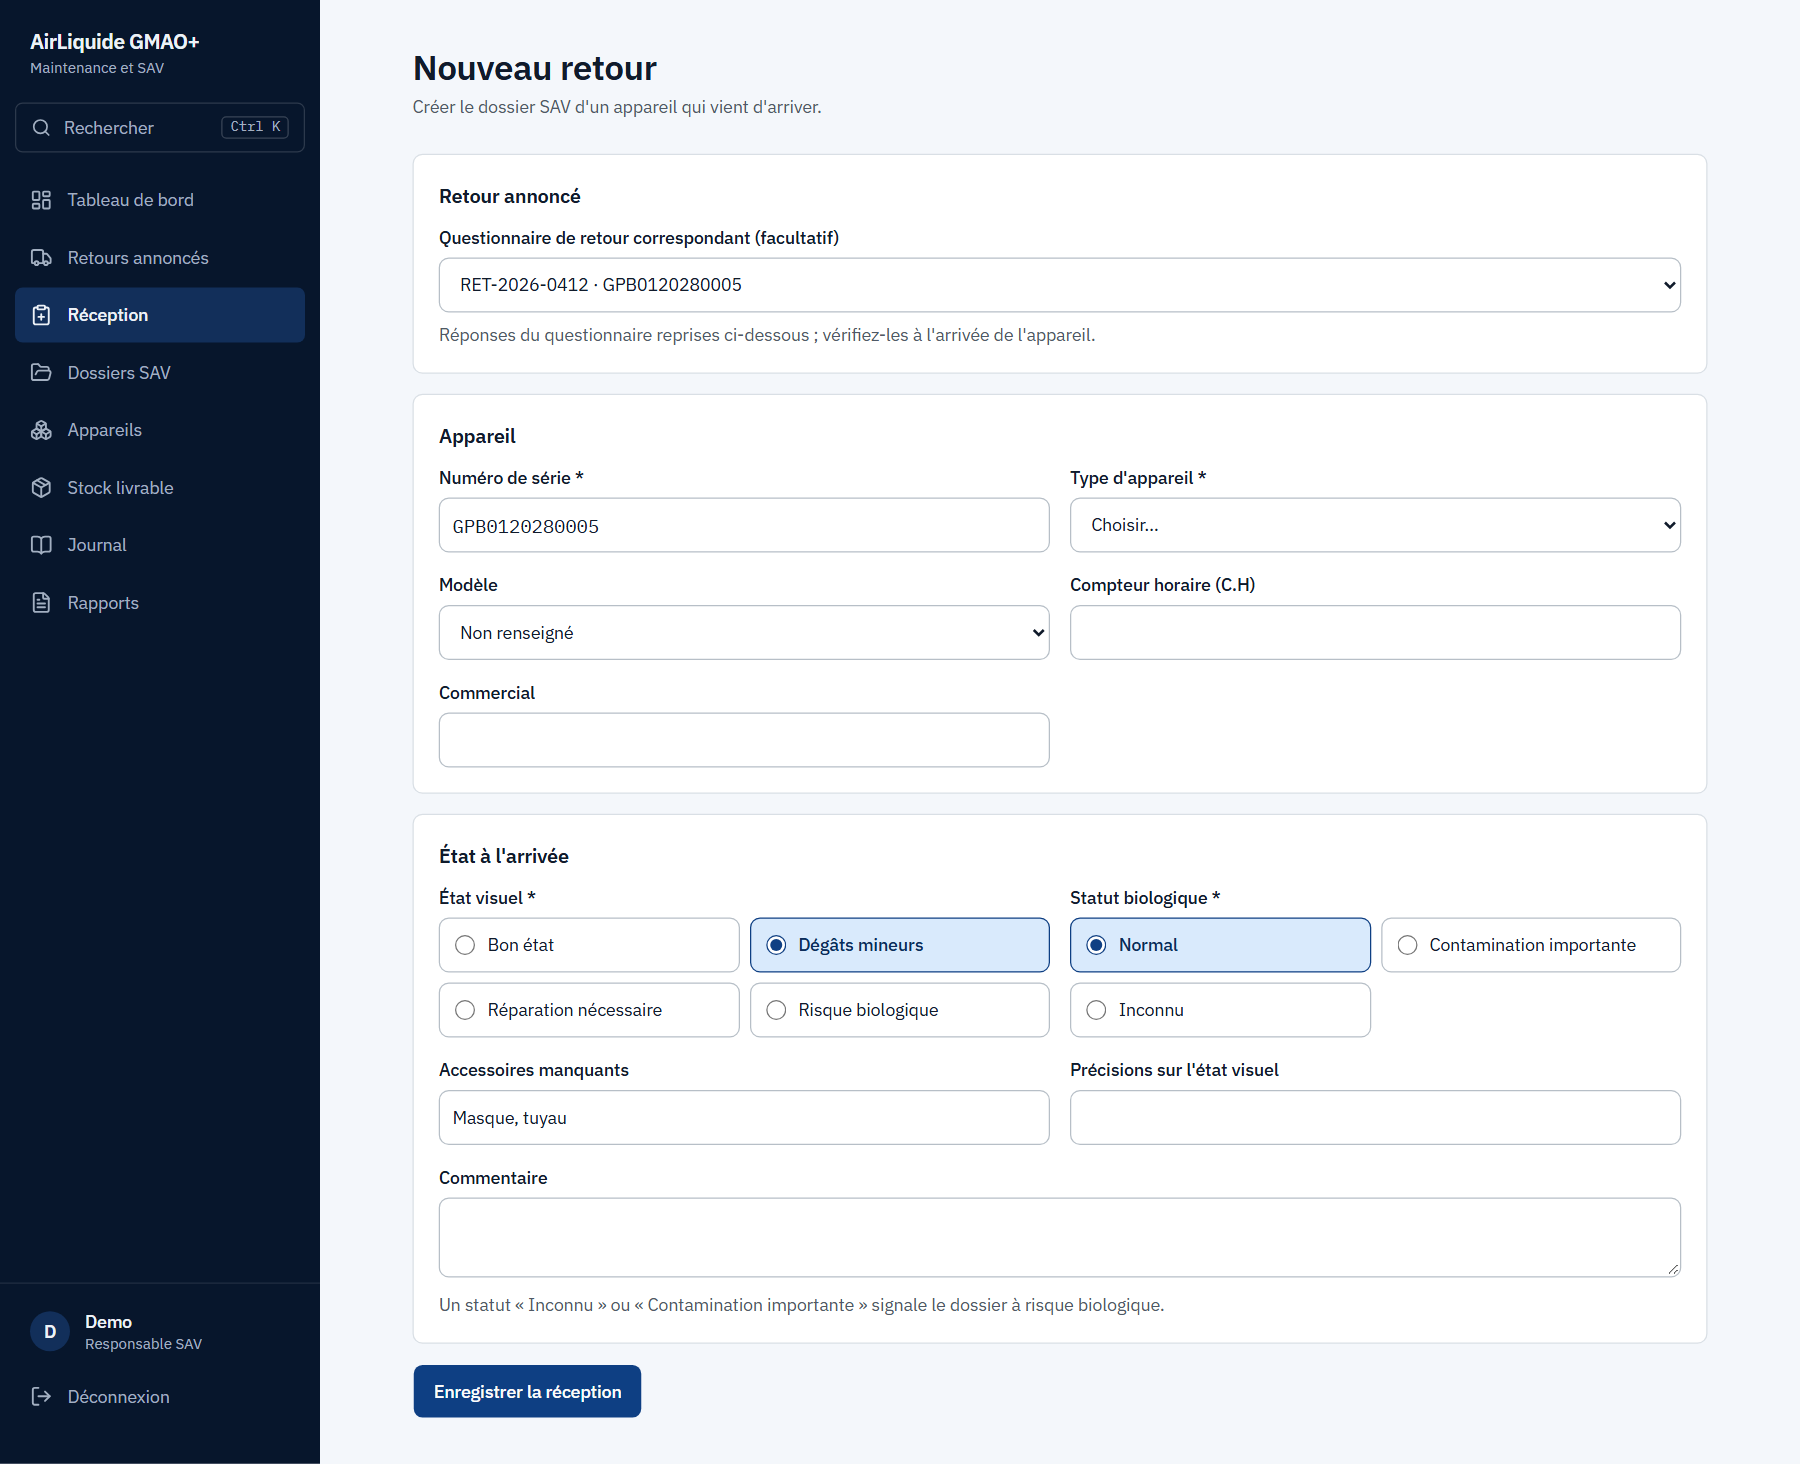
\includegraphics[width=14.0cm,height=17.5cm,keepaspectratio]{cap_reception.png}
\caption{Écran de réception d'un appareil (données de démonstration)}
\end{figure}

\subsection{Le journal de maintenance}

Le registre papier a été reproduit sous forme numérique. Le journal n'est \textbf{pas une table à saisir} : il est calculé à partir des dossiers, une ligne par retour, avec les douze colonnes du registre (annexe D). Il ne peut donc pas diverger des dossiers. L'écran propose des filtres (année, mois, type, numéro de série), l'impression et l'export CSV. Pour alimenter les colonnes du registre, le compteur horaire est saisi à la réception ; la pureté, le débit ou la pression et l'alarme sonore au contrôle qualité ; le document de sortie des pièces à la réparation.

\begin{figure}[!htb]
\centering
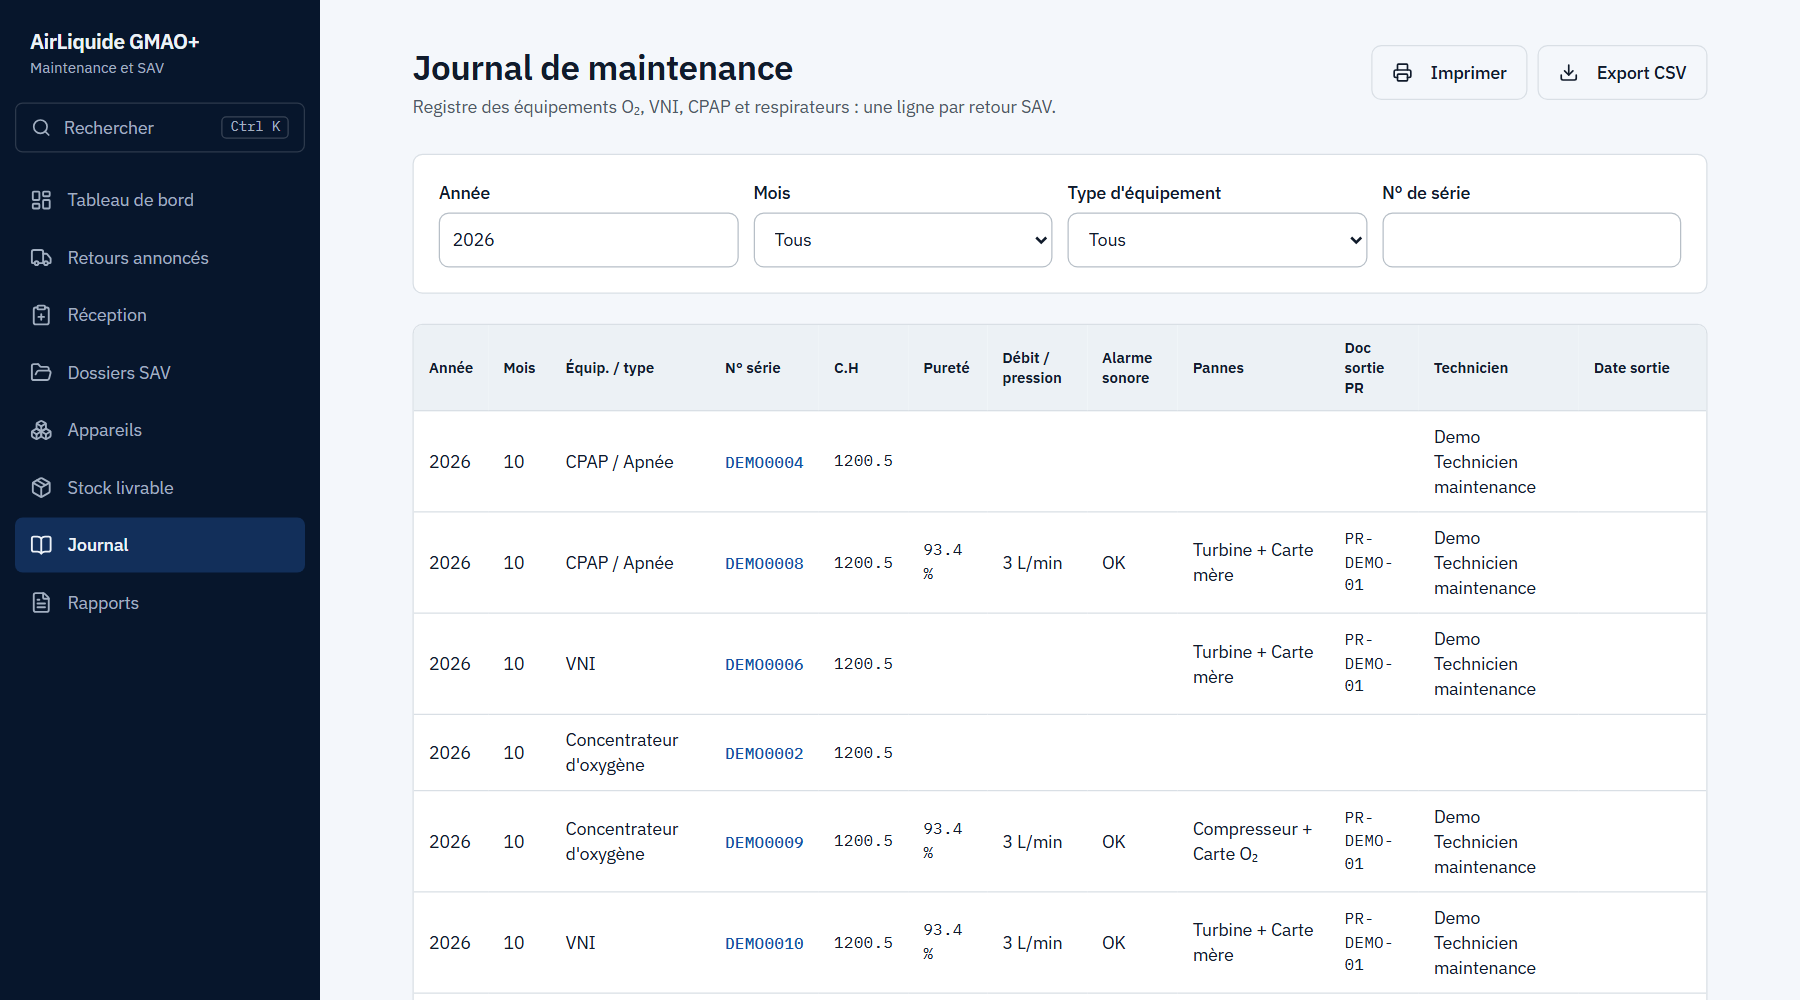
\includegraphics[width=15.0cm,height=17.5cm,keepaspectratio]{cap_journal.png}
\caption{Journal de maintenance numérique (données de démonstration)}
\end{figure}

\subsection{Le frontend et l'expérience utilisateur}

L'interface est en français et vise l'usage en atelier : cibles tactiles d'au moins 44 pixels, contrastes suffisants, statuts toujours accompagnés d'un libellé et d'une icône (jamais la couleur seule), navigation au clavier. Plusieurs choix répondent à des besoins observés :

\begin{itemize}
  \item le \textbf{tableau de bord} montre la charge de l'atelier par poste (à désinfecter, à diagnostiquer, etc.) et la liste des dossiers à traiter en premier, du plus ancien au plus récent ;
  \item le \textbf{dossier} est présenté comme un parcours vertical : les étapes terminées se résument sur place et le formulaire de l'étape en cours s'ouvre à sa position ;
  \item la \textbf{recherche rapide} (Ctrl + K) retrouve un appareil par son numéro de série ;
  \item des \textbf{confirmations} (notifications) signalent chaque enregistrement ; les erreurs sont expliquées en clair.
\end{itemize}

\begin{figure}[!htb]
\centering
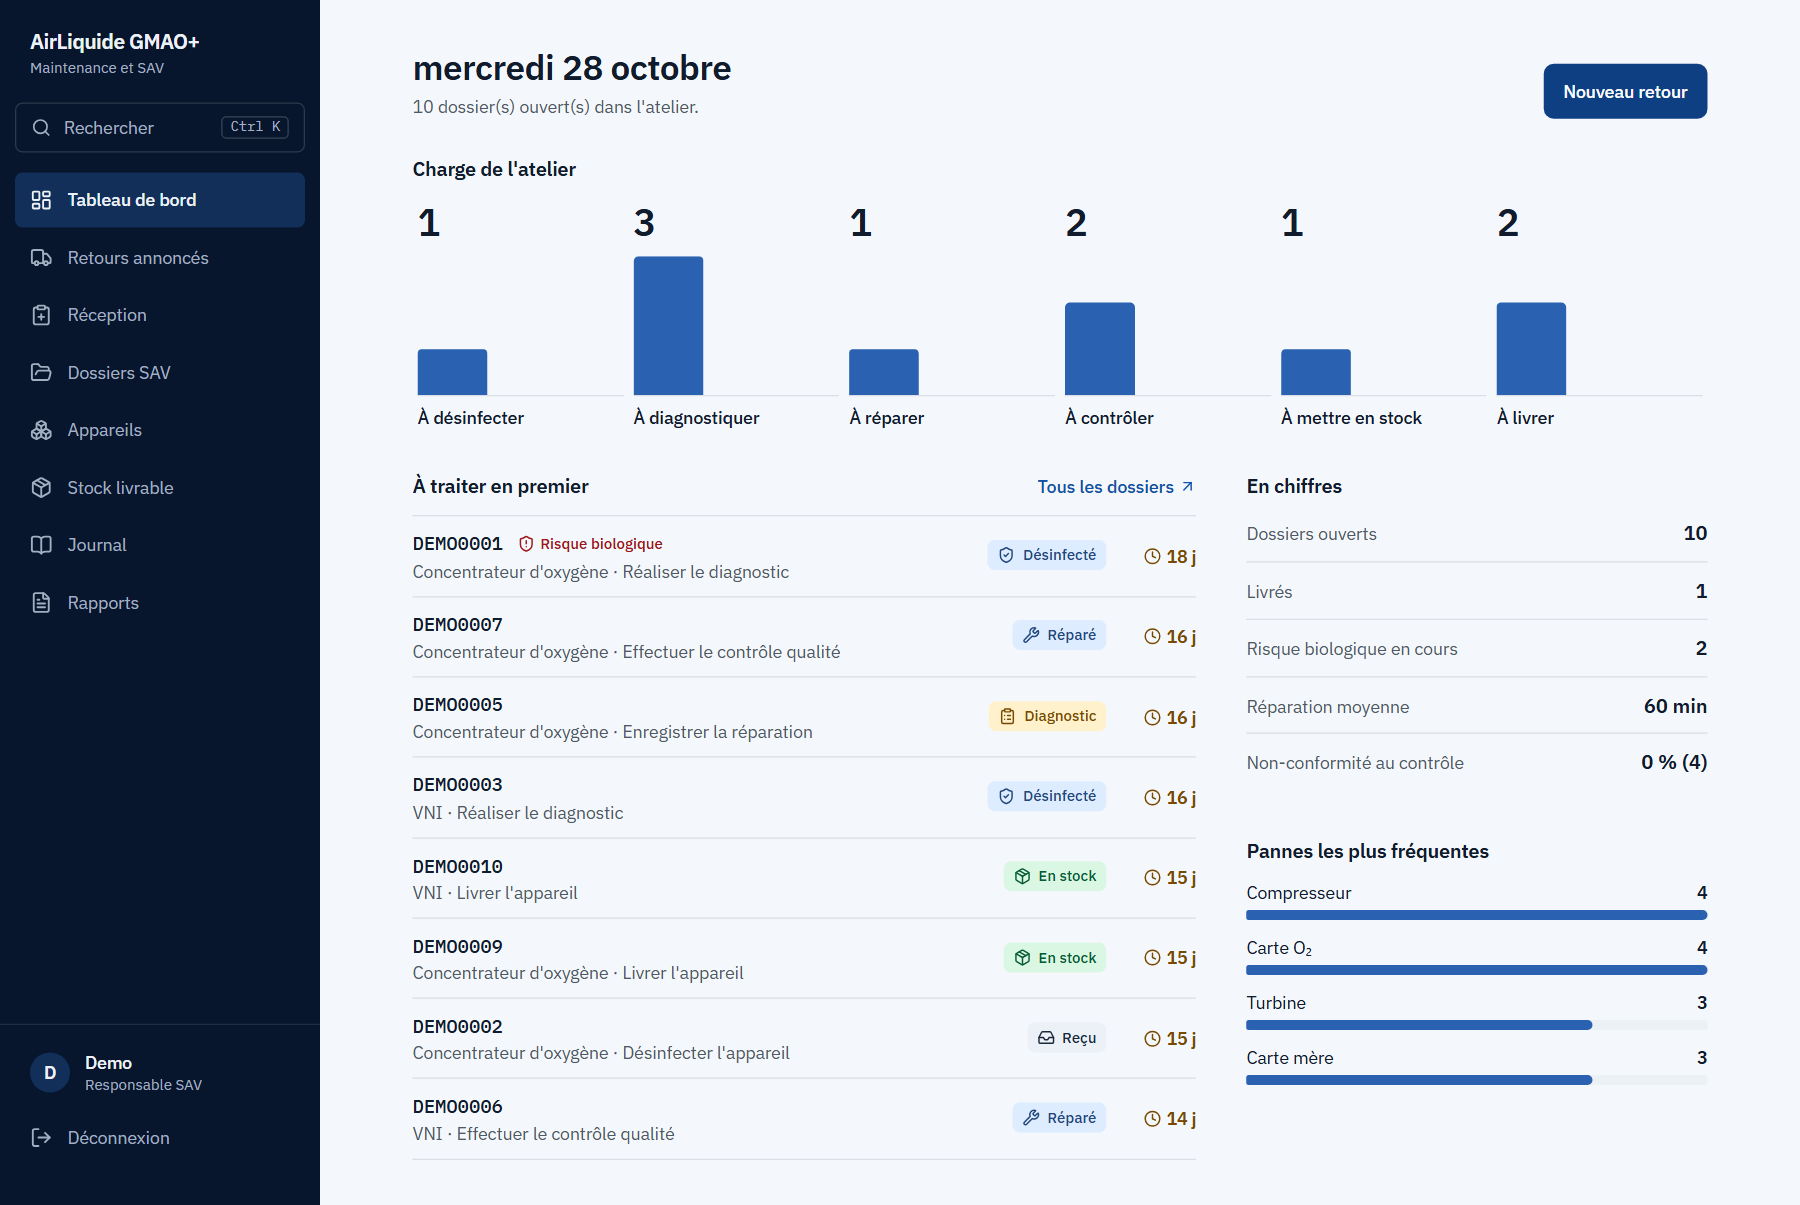
\includegraphics[width=15.5cm,height=17.5cm,keepaspectratio]{cap_tableau_de_bord.png}
\caption{Tableau de bord (données de démonstration)}
\end{figure}

\begin{figure}[!htb]
\centering
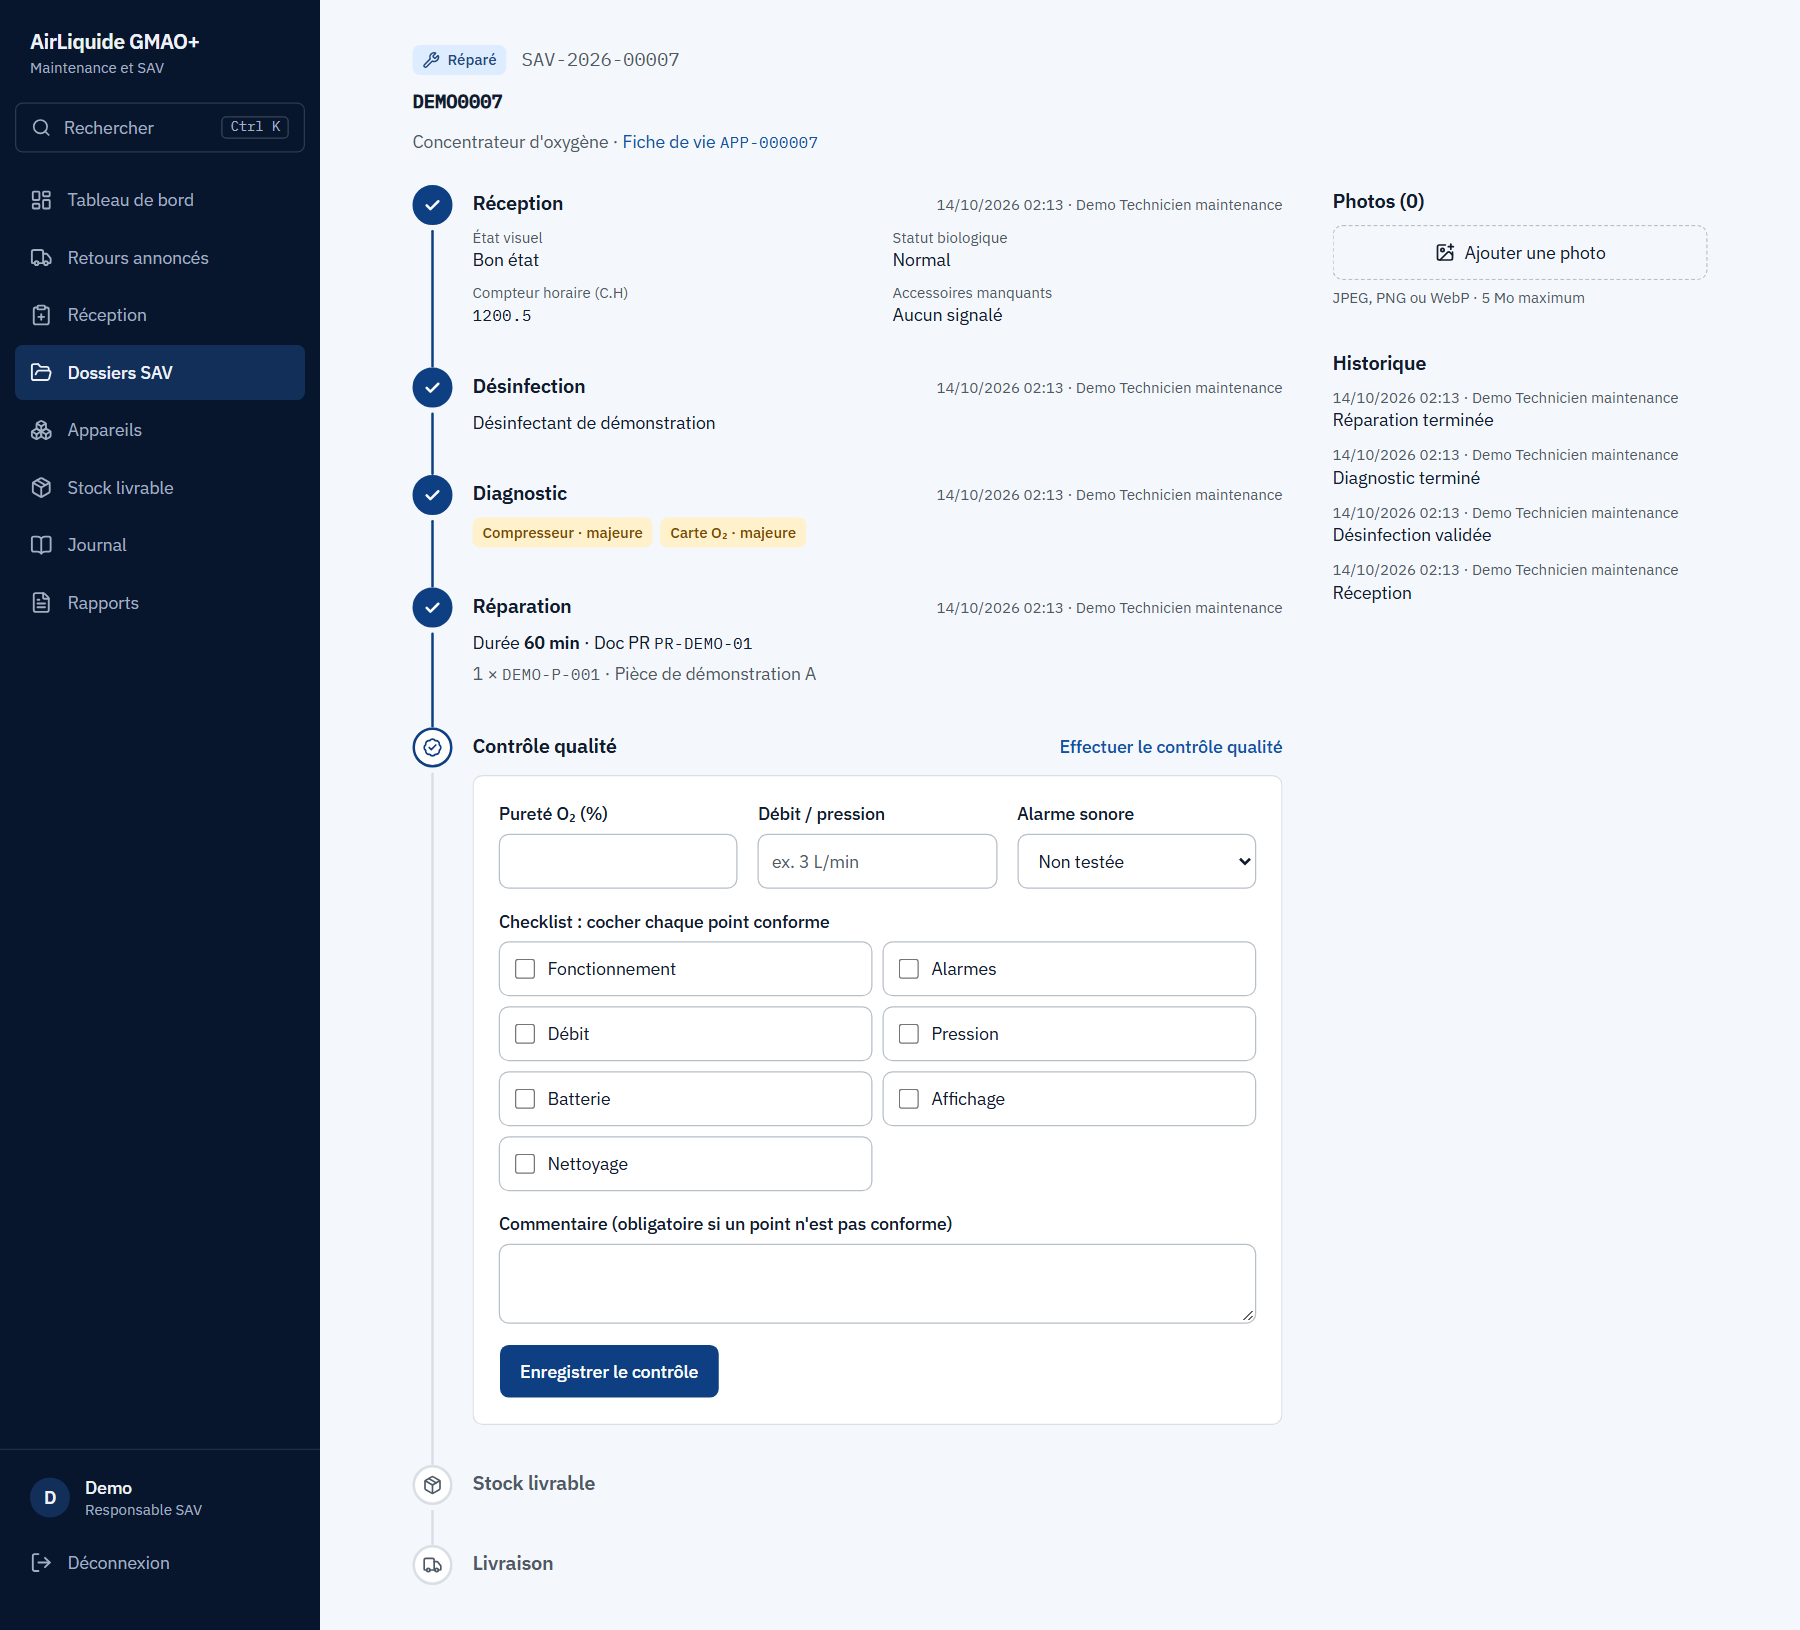
\includegraphics[width=15.0cm,height=17.5cm,keepaspectratio]{cap_dossier_qc.png}
\caption{Dossier SAV : parcours et formulaire de contrôle qualité}
\end{figure}

\begin{figure}[!htb]
\centering
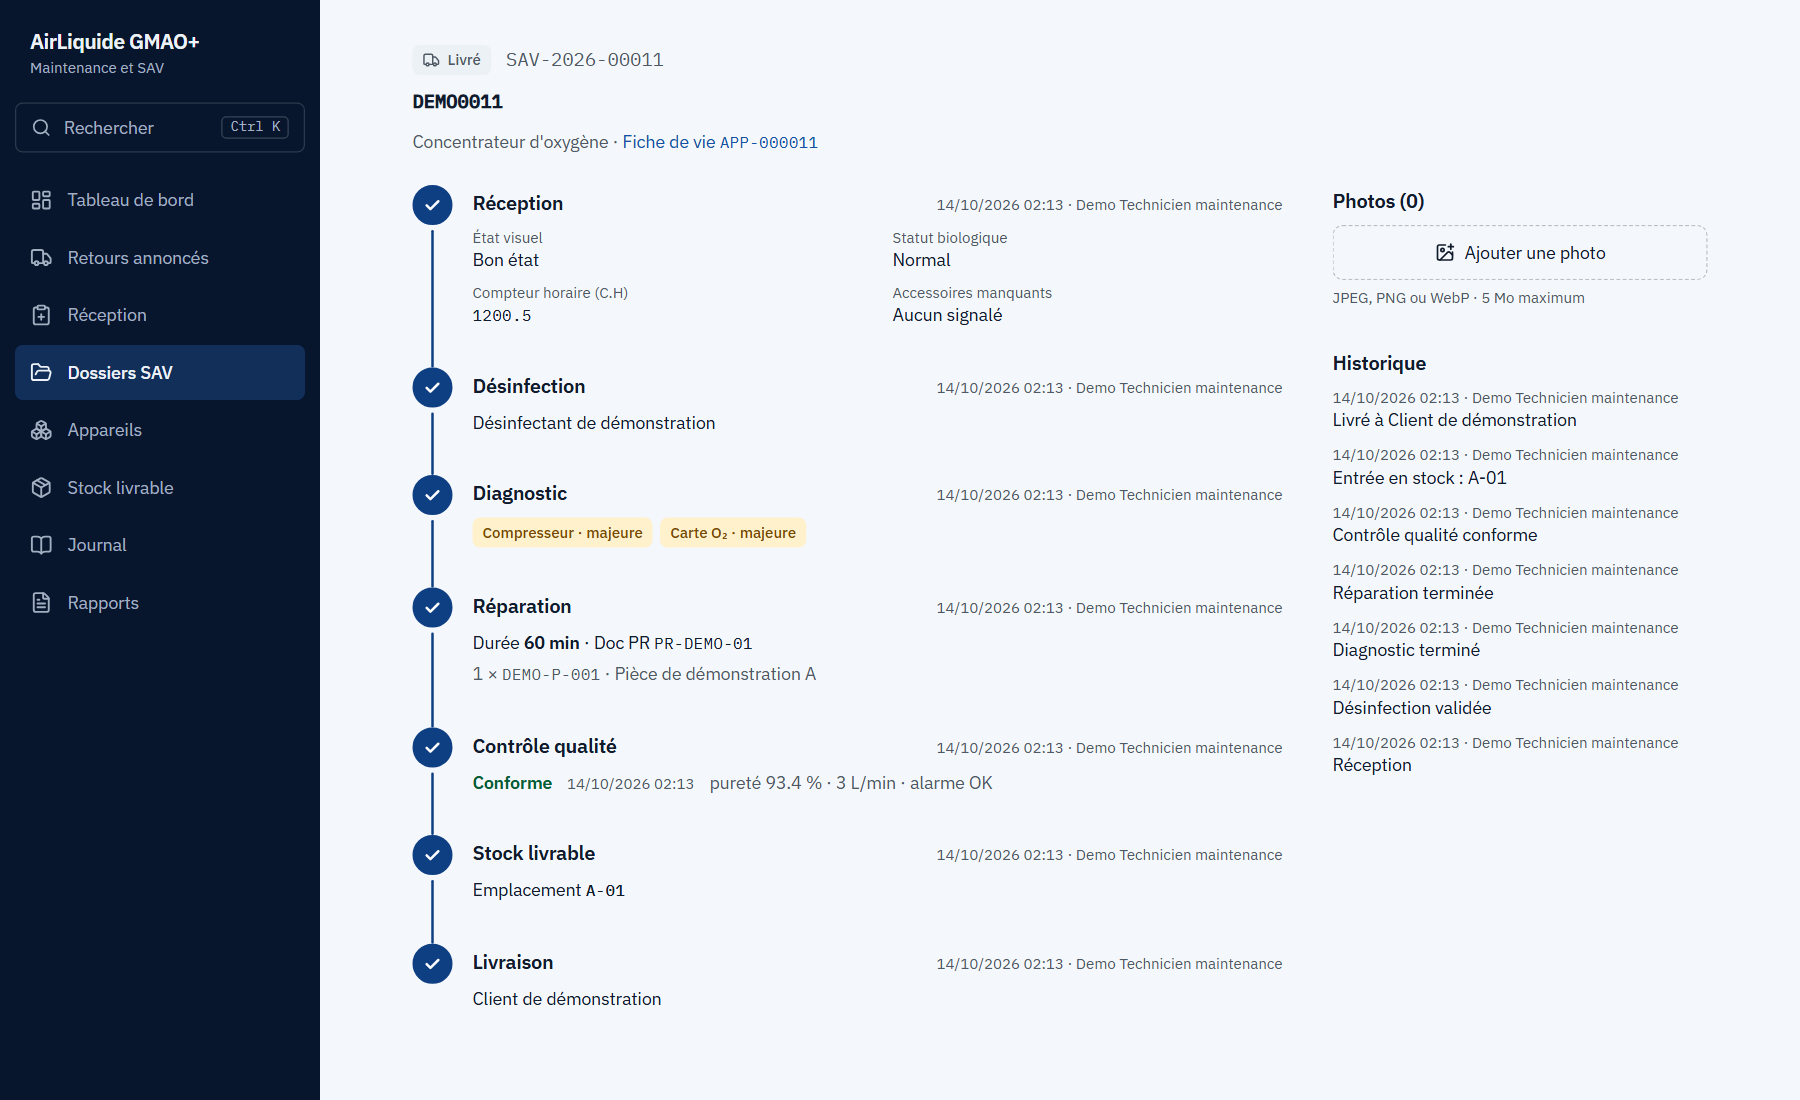
\includegraphics[width=15.0cm,height=17.5cm,keepaspectratio]{cap_dossier_livre.png}
\caption{Dossier livré : toutes les étapes sont résumées}
\end{figure}

Les captures de ce rapport ont été réalisées avec des \textbf{données de démonstration fictives}, clairement identifiées, et non avec des données réelles d'Air Liquide.

